\documentclass[a4wide,12pt]{book}

\usepackage[swedish,english]{babel} % Use English and Swedish languages. English default. English hyphenation.
\usepackage{amsmath,amsfonts,amsthm} % Math packages
\usepackage{bm}
\usepackage{txfonts}
\usepackage{graphicx}
\usepackage{wrapfig}
\usepackage{caption}
\usepackage{sidecap}
\usepackage{subcaption}
\usepackage{float}
\usepackage{epstopdf}
\usepackage{titlesec}
\usepackage{verbatim}
\usepackage{amssymb}
\usepackage{natbib}
\bibpunct{(}{)}{;}{a}{}{,}     %% natbib format like A&A and ApJ
\usepackage{fancyhdr}
\pagestyle{fancy}
\usepackage{enumerate}
\usepackage[Lenny]{fncychap}
\usepackage[font={small,it}]{caption}
\usepackage{footnote}
\usepackage{url}

\makeatletter
\def\cleardoublepage{\clearpage\if@twoside \ifodd\c@page\else
\hbox{}
\thispagestyle{empty}
\newpage
\if@twocolumn\hbox{}\newpage\fi\fi\fi}
\makeatother

\pagenumbering{roman}

\setlength{\hoffset}{-0.5cm}
\setlength{\textwidth}{38pc}
\setlength{\textheight}{52pc}
\setlength{\oddsidemargin}{3.5mm}
\setlength{\evensidemargin}{3.5mm}
\setlength{\topmargin}{7mm}

%Biblio
\def\aj{AJ}%
          % Astronomical Journal
\def\araa{ARA\&A}%
          % Annual Review of Astron and Astrophys
\def\apj{ApJ}%
          % Astrophysical Journal
\def\apjl{ApJ}%
          % Astrophysical Journal, Letters
\def\apjs{ApJS}%
          % Astrophysical Journal, Supplement
\def\ao{Appl.~Opt.}%
          % Applied Optics
\def\apss{Ap\&SS}%
          % Astrophysics and Space Science
\def\pasp{PASP}%
          % Publications of the ASP
\def\aap{A\&A}%
          % Astronomy and Astrophysics
\def\aapr{A\&A~Rev.}%
          % Astronomy and Astrophysics Reviews
\def\aaps{A\&AS}%
          % Astronomy and Astrophysics, Supplement
\def\mnras{MNRAS}%
          % Monthly Notices of the RAS
\def\nat{Nature}%
          % Nature

\def\pasa{PASA}
\newcommand{\msun }{$\mathrm{M}_{\odot}$}
\newcommand{\ignore}[1]{}

\begin{document}

\titlepage
\begin{center}

\begin{figure}[!h]
\vspace{-1.5cm}

\includegraphics[width=0.15\textwidth]{SU-Logga.eps}
\end{figure}
\textit{\Large{Stockholm University}}\\

\Large{Department of Astronomy}\\

\vspace{1.5cm}
\large{LICENTIATE THESIS}\\

\vspace{0.1cm}

{\bf \LARGE{Gravitational lensing and radio interferometry as a probe of the small--scale structure of dark matter\\ \vspace{1.4cm} }}~\\
\end{center}

\vspace{-1.0cm}
\begin{center}
\large{{\it Author:}\\ Saghar Asadi}\\
\vspace{0.5cm}
\small{\it Department of Astronomy,\\ The Oskar Klein Center,\\ Stockholm University,\\ AlbaNova,\\ 106 91 Stockholm,\\ Sweden}

\vspace{1.0cm}
\large{{\it Supervisor:}\\ Erik Zackrisson}\\
\vspace{0.5cm}
\large{{\it Co-Supervisors:}\\ Emily Freeland\\ Garrelt Mellema}\\
\vspace{0.5cm}
\end{center}

\vspace{1.2cm}

\begin{center}
\large{Jan 11, 2016}\\
\end{center}
\thispagestyle{empty}
\fancyhf{}
\fancyhead{}
\rule[1cm]{0cm}{0.0cm} \\
\scriptsize{\emph{}\\
\clearpage
\normalsize
\pagenumbering{arabic}
\fancyhf{}
\fancyhead{}

\renewcommand{\chaptername}{}
\renewcommand{\chaptermark}[1]{\markboth{#1}{}}
\fancyhead[LO]{\it \textbf{\thechapter . \leftmark}}
\renewcommand{\sectionmark}[1]{\markright{#1}{}}
\fancyhead[RE]{\it \textbf{ }}

\fancyhead[LE]{\thepage}
\fancyhead[RO]{\thepage}

\renewcommand{\headrulewidth}{0.4pt}



\chapter*{List of acronyms}

\begin{description}
\item[ALMA]
Atacama Large Millimeter/sub--millimeter Array
\item[BL]
Base Line
\item[CASA]
Common Astronomy Software Applications \footnote{The software can be downloaded from \url{http://casa.nrao.edu/}}
\item[CDM]
Cold Dark Matter
\item[DM]
Dark Matter
\item[EVN]
European VLBI Network
\item[GL]
Gravitational lensing
\item[IMBH]
Intermediate--Mass Black Hole
\item[NFW]
Navarro--Frenck--White, the Universal density profiles of simulated CDM halos, first introduced by \citet{NFW}
\item[SMG]
Sub--Millimeter Galaxy
\item[UCMH]
UltraCompact MiniHalo
\item[VLBI]
Very Long Baseline Interferometry
\item[WIMP]
Weakly--Interacting Massive Particle
\end{description}

\clearpage

\chapter*{Abstract}
\thispagestyle{empty}
\emph{Gravitational lensing} has been used to study otherwise faint and unresolved objects for about a century.The fact that gravity treats dark and luminous mass the same way, gives GL a unique advantage over many other observational methods to provide an independent test for the presence of dark structures of various size and mass. Strong lensing by a foreground object can produce multiple images of a background light source, known as \emph{macroimages}. Measurements of strong lens systems provide information about mass distribution of both the lens and the source. On the other hand, the concordance model of cosmology\ignore{ -- accounting for dark matter as the second abundant component in the Universe --} has yet to describe the observed Universe at different scales simultaneously. one way to probe the small--scale structures in dark matter is to look at a particular type of lens system where the foreground galaxy produces multiple images of the background light source, and the halo substructure presents itself as a surface brightness perturbation in one of the macroimages.

Revealing small--scale surface brightness perturbations requires high--resolution imaging of lensed extended sources. Radio interferometry is a technique that connects an array of radio antennae to essentially work as a single dish with the diameter as large as the maximum distance within the array. Arrays such as the VLBI network or ALMA, or combinations of these, make it possible to probe radio quasars and SMGs with sub--milliarcsecond angular resolutions.

In this thesis, we simulate observations of multiply--lensed sources (radio quasars and dusty star--forming galaxies) at $z \simeq 2$ with different (present and near--future) radio interferometers. These simulations are used to place constraints on various forms of suggested halo substructures within the lens halo. In {\bf Paper I}, we derive the minimum  mass that subhalos with different internal density profiles need to have in order to produce detectable lensing effects on multiply--imaged quasars using three different radio arrays. Using the derived minimum detectable mass of different forms of subhalos, we estimate constraints that observations of a number of such lens systems can place on the contribution of each form of substructure in the mass of the parent halo. {\bf Paper II} focuses on simulations of SMGs using ALMA and the prospects for detecting standard CDM subhalos. In this paper, we show that standard CDM subhalos in the sub--galactic mass range are detectable using high--frequency observations with ALMA. In addition to probing the mass of the substructure such observations are able to discern the difference between the standard CDM subhalos and other dark compact objects.  This can place constraints on the contribution of CDM subhalos to the mass of their host halo -- a quantity directly comparable to cosmological simulations.


%Dark matter has been one of the great mysteries of physics for several decades now. Despite numerous constraints on the properties of dark matter, the concordance model of cosmology\ignore{ -- accounting for dark matter as the second abundant component in the Universe --} has yet to describe the observed Universe at different scales simultaneously.

%One property of gravity that has been known and used for a long time is \emph{gravitational lensing}. The fact that gravity treats dark and luminous mass the same way, gives GL a unique advantage over many other observational methods to provide an independent test for the presence of dark structures of various size and mass. Strong lensing by a foreground object can produce multiple images of a background light source, known as \emph{macroimages}. Measurements of strong lens systems provide information about mass distribution of both the lens and the source. One way to study the structure inside dark matter halos of galaxies is to look at a particular type of lens system where the foreground galaxy produces multiple images of the background light source, and the halo substructure presents itself as a surface brightness perturbation in one of the macroimages.

%Revealing small--scale surface brightness perturbations requires high--resolution imaging of a lensed extended object, such as star--forming galaxies and radio jets. Radio interferometry is a technique that connects an array of radio antennae to essentially work as a single dish with the diameter as large as the maximum distance within the array. Arrays such as the VLBI network or ALMA, and different combinations of these arrays, make it possible to probe radio quasars and sub--mm galaxies with sub--milliarcsecond angular resolutions.

%In this thesis, we simulate observations of multiply--lensed sources (radio quasars and dusty star--forming galaxies) at $z \simeq 2$ with different (present and near--future) radio interferometers. These simulations are used to place constraints on various forms of suggested halo substructures within the lens halo. In {\bf Paper I}, we derive the minimum  mass that subhalos with different internal density profiles need to have in order to produce detectable lensing effects on multiply--imaged quasars using three different radio arrays. Using the derived minimum detectable mass of different forms of subhalos, we estimate constraints that observations of a number of such lens systems can place on the contribution of each form of substructure in the mass of the parent halo. {\bf Paper II} focuses on simulations of SMGs using ALMA and the prospects for detecting standard CDM subhalos. In this paper, we show that standard CDM subhalos in the sub--galactic mass range are detectable using high--frequency observations with ALMA. In addition to probing the mass of the substructure such observations are able to discern the difference between the standard CDM subhalos and other dark compact objects.  This can place constraints on the contribution of CDM subhalos to the mass of their host halo -- a quantity directly comparable to cosmological simulations.


\clearpage

\thispagestyle{empty}

\section*{List of papers and my contribution}
  \begin{enumerate}[I]
    \subsection*{Included in this thesis}
      \item Zackrisson, E.; {\bf Asadi, S.}; Wiik, K.; J{\"o}nsson, J.; Scott, P.; Datta, K.K.; Friedrich, M.M.; Jensen, H.; Johansson, J.; Rydberg, C--E.; Sandberg, A.;  Monthly Notices of the Royal Astronomical Society, Volume 431, Issue 3, p.2172-2183 \\{\it Hunting for dark halo substructure using submilliarcsecond-scale observations of macrolensed radio jets}\\
      I ran all simulations and generated all figures in this paper and contributed to the text.
      \item {\bf Asadi, S.}; Zackrisson, E.; Freeland, E.; submitted\\{\it Probing cold dark matter subhalos with simulated ALMA observations of macrolensed sub–mm galaxies}\\
      All the simulations and modellings in the paper are done by me. I also wrote the text.
      
    \subsection*{Other papers}
%      \item Amanullah, R.; [28 co--authors]; {\bf Asadi, S.};  [9 co--authors]; Monthly Notices of the Royal Astronomical Society, Volume 453, Issue 3, p.3300-3328 \\{\it Diversity in extinction laws of Type Ia supernovae measured between 0.2 and 2 $\mu$m}\\
%      I was one of the observers. The observations of SN? was done remotely by the Nordic Optical Telescope (NOT) during a summer school I was attending.
      \item Zackrisson, E.; Calissendorff, P.; {\bf Asadi, S.}; Nyholm, A.; The Astrophysical Journal, Volume 810, Issue 1, article id. 23, 12 pp. (2015)\\{\it Extragalactic SETI: The Tully-Fisher Relation as a Probe of Dysonian Astroengineering in Disk Galaxies}\\
      The simulations presented in this paper are made by me. I also contributed to the text about the simulation part of the paper.
      \item Zackrisson, E.; González, J.; Eriksson, S.; {\bf Asadi, S.}; Safranek--Shrader, C.; Trenti, M.; Inoue, A.K.; Monthly Notices of the Royal Astronomical Society, Volume 449, Issue 3, p.3057--3063\\{\it Primordial star clusters at extreme magnification}\\
      {\bf I ran lensing simulations of highly--magnified galaxies as seen by JWST as a proof--of--concept!}
      \item Rydberg, C--E.; Zackrisson, E.; Zitrin, A.; Guaita, L.; Melinder, J.; {\bf Asadi, S.}; Gonzalez, J.; {\"O}stlin, G.; Str{\"o}m, T.; The Astrophysical Journal, Volume 804, Issue 1, article id. 13, 16 pp. (2015)\\{\it A Search for Population III Galaxies in CLASH. I. Singly--imaged Candidates at High Redshift}\\
      Color--color diagrams (Figure 2) are made by me.
      \item Tilanus, R. et al.; White paper; eprint arXiv:1406.4650\\{\it Future mmVLBI Research with ALMA: A European vision}
  \end{enumerate}

\tableofcontents

\thispagestyle{empty}

%%  ------------------------  %%
\chapter{Dark matter}
\pagenumbering{arabic}
Dark matter, the second dominant component of our Universe, is thought to be made of non--baryonic, cold (i.e. non--relativistic), weakly interacting massive particles (WIMPs). Some of these characteristics are inferred from cosmological evidence. For instance, observations of small--scale cosmic structure indicate that dark matter must be non--relativistic.  The measured abundance of light elements in the Universe, along with Big Bang Nucleosynthesis (BBN) results in dark matter being non--baryonic. This ``missing matter'' in the Universe has presented itself both locally, i.e. in the Galactic disk, and at the cosmic scale in the past century. Even though the problem has been approached from the particle--physics point of view in addition to the cosmological one, it is still considered as one of the biggest challenges of both!

I start this chapter by describing independent cosmological evidences for the presence of dark matter (in order of decreasing physical scale which does not necessarily correspond to historical order) and what each of them tells us about the nature and characteristics of dark matter. The chapter is finished by a review of the current state of dark matter followed by the detection methods currently used to approach the issue.

Modern data suggests an insignificant amount of dark matter in the Solar vicinity which is made of baryonic but not luminous matter such as faint stars or Jupiter--like objects. In short, according to our current understanding of the Universe, dark matter is the dominant matter component of the Universe.

\section{Why do we need dark matter?}
The amount of baryons in the Universe can be measured with five independent methods, all of which result in a fraction less than 5\% of the total content of the Universe. From the abundance of light elements in BBN, to anisotropies in the angular power spectrum of the cosmic microwave background, to the X--ray emission from galaxy clusters leading to an estimation of their baryon fractions, and the discrepancies between the dynamical mass and luminous mass of galaxies, the Universe seems to be full of discrepancies that can be resolved by adding the missing mass in a non--baryonic form. Although, it is worth mentioning that these observations can be interpreted differently, leading to alternative theories of gravity that will not be covered in this thesis \citep[but see e.g. ][]{Clifton2006, Clifton+2012, Bloomfield2013}.

\subsection{CMB temperature fluctuations}
\label{subsec:CMB}
Structures in the Universe are believed to have grown from small fluctuations in the primordial density field after the era of recombination. Density fluctuations are of the same order as temperature fluctuations, therefore measuring temperature fluctuations of the CMB reveals the order of magnitude of density fluctuations in the early Universe. However, taking only the baryonic matter into account, these fluctuations are too small to give rise to any structure formation in our expanding Universe. While the required amount of matter in the Universe, in units of the critical cosmological density, is $\Omega_m \equiv \rho/\rho_\mathrm{crit}\sim 0.3$ the estimated upper limit for the baryonic matter density parameter $\Omega_b$ is $ \sim 0.025$ \citep[][]{Planck2015} supporting the non--baryonic nature of dark matter. Moreover, if dark matter is non--baryonic, its density fluctuations can start growing already at the radiation--dominated era while the growth of baryonic matter is damped by radiation. After the decoupling of baryons and photons, baryons collapse into the local potential minima mainly generated by the dark matter perturbations and form cosmic structures. The importance of the CMB is that it may serve as a probe to the state of the Universe at the time of the last scattering, as well as the age and conditions of the Universe ever since.

\subsection{Gravitational lensing}
The mathematical framework of gravitational lensing has been a commonly accepted framework in astronomy for a long time. However, evidence for dark matter arose only after the general relativistic corrections to the Newtonian formalism of gravitational lensing. Gravitational lensing, as an accurate and reliable gravitational mass measurement of the lens, confirmed the discrepancy between the gravitational and luminous mass both on galactic and galaxy cluster scales. Gravitational lensing is now a common technique in astrophysics, and also widely used in my project. This makes it worth a section of its own: \S \ref{sec:Gravitational lensing}.

\subsection{Masses of galaxy clusters}
In the beginning of the 1930s, Zwicky was first to notice the order--of--magnitude difference between the dynamical mass of the Coma cluster and the mass in luminosities of individual galaxies \citep[][]{Zwicky1933}. The discrepancy was not recognized as an issue until after its persistence in various observations \citep[][]{Rubin.Ford1970, Einasto+1974, Ostriker+1974}. X--ray observations of hot gas in galaxy clusters confirmed that the hot gas reservoir cannot explain the missing mass. The X--ray data, additionally, provided new measurements of the velocity dispersions of galaxies in clusters, confirming the previous dynamical mass estimates\ignore{(Forman et al. 1972, Gursky et al. 1972, Kellogg et al. 1973)}. The previously unknown population of dark (or high mass--to--light ratio) matter was now accepted to dominate the mass budget of the Universe. The mean density of the matter was shown to be $\sim 0.2$ of the critical density of the Universe and different models for dark matter started appearing in the literature. Firstly, the missing matter was thought to be in faint stars or hot gas but both failed to explain the situation\ignore{cite and explain why! or maybe not as it's not really important now!!}. The first non--baryonic candidate for dark matter particles was the neutrino. However, simulations based on this model \citep[][]{Doroshkevich+1978} indicated that neutrino--dominated dark matter cannot give rise to small scale structure in the distribution of galaxies due to the cut--off of the power spectrum of these rapidly--moving particles. This also suggested that suitable candidates for dark matter particles not only need to be dissipationless, but are also required to be much more massive than neutrinos\ignore{(Blumenthal et al. 1982, Bond et al. 1982, Peebles, 1982)}. Therefore, the first numerical cosmological simulations based on cold dark matter CDM were performed by \citep[][]{Melott+1983} and these were able to represent the small structures of the Universe much more accurately.

\subsection{Galactic rotation curves}
The first galaxy that showed an increasing mass profile to very large radii was M31 \citep[][]{Rubin.Ford1970}. By the next decade, both optical\ignore{ (Rubin+1978, Rubin+1980)} and radio\ignore{ (Bosma 1978)} data had confirmed the flat rotational curves of disk galaxies at large radii. It was the deep and high resolution HI observations that proved the flat rotation curves of a large number of galaxies beyond the optical disk, providing important evidence for the presence of massive halos around galaxies. \citet[see e.g.][]{Bosma1981, Begeman1989}. 

\section{What do we know about dark matter?}
\label{subsec:current state}
The commonly--accepted class of DM particles are Weakly Interacting Massive Particles (WIMPs). The main characteristics of WIMPs are listed below:
  \begin{itemize}
  \item {\bf Heavy} -- \ignore{The observational upper and lower bounds for dark matter particles come from different sources. }While the upper limit is placed by undetection of MACHOs (Massive Astrophysical Compact Halo Objects), the lower limit is far less constrained.\ignore{ Neither the Kepler satellite \citep[][]{Griest+2014}, nor microlensing surveys \citep[][]{Alcock+1998, Yoo+2004} did not detect MACHOs as predicted.} These limits expect the DM particle mass to be between $10^\mathrm{-31} GeV (= 9\times 10^\mathrm{-89}$\msun  $) < m < 2\times 10^\mathrm{48} GeV (= 2 \times 10^\mathrm{-9}$\msun ) \citep[\ignore{47 for lower bound}][\ignore{ and 42 \& 43 for the upper bound}]{Hu+2000, Alcock+1998, Yoo+2004}. Note the 80 orders of magnitude mass range. This is how much we know about the second most abundant component in our Universe!
  \item {\bf Dissipationless and collisionless} -- The existence of dark matter halos around galaxies is evidence for the dark matter to be dissipationless. Being dissipationless means that dark matter cannot cool by emitting photons like baryons do. Therefore, while dark matter comes together and forms extended halos, baryonic matter falls into the gravitational well of these halos and cools down by emitting photons and then forms stars and galaxies at the halo center. Dark matter is also assumed to be collisionless, meaning that it does not interact with other dark matter particles. An upper limit on the cross section of dark matter comes from the famous case of the Bullet cluster \citep[][]{Clowe+2006}. The collisionless property of dark matter can alleviate two of the small--scale challenges to the CDM model that I discuss in the next section; the cusp--core problem \ref{subsec:core-cusp}, and the too--big--to--fail problem \ref{subsec:too-big-to-fail}.
  \item {\bf Cold} -- the terms ``cold'', ``warm'', and ``hot'' dark matter refer to the mass of the dark matter particles which is the deciding factor in their velocity at the freeze--out epoch. This is the time when the temperature of the Universe decreased to $\sim 10^9$ K. At this temperature, hot DM particles that are light are relativistic. Therefore small density perturbations do not survive, i.e. the early structures that form in the Universe are superclusters. Smaller structures such as galaxy cluster, galaxies and dwarf galaxies form via fragmentation, but this does not match our observations. However, if dark matter particles are as described by cold DM or warm DM structure formation follows a bottom--up hierarchy where small scale structures (down to dwarf galaxies in case of WDM and even smaller fluctuations in case of CDM survive). These small structures then merge/fall into the potential wells of larger growing structures. 
  \end{itemize}


%%  ------------------------  %%
\chapter{The standard model of cosmology; strengths and challenges}
\label{sec:LCDM}
Dark matter seems to be dominating the matter content of our Universe. Our best model for dark matter particles are WIMPs whose interaction with themselves or baryons are limited to gravity.  WIMPs do not cool by emitting photons as baryons do (see subsection \ref{subsec:current state}). Therefore, cosmic structure formation at large scales is thought to be dominated by the behavior of dark matter. Baryonic effects, however, are only thought to dominate the observable Universe at scales of galaxies and below where the energy content of hydrodynamical effects such as supernovae and black hole jets are sufficient to alter their environment. The most common way to perform cosmological N--body simulations has been to simulate a pure dark matter Universe without including the complex physics of the baryonic matter.  Even though this approach provides a consistent picture of our Universe on large scales, it faces systematic inconsistencies when describing scales of galaxies and below. The physics of baryonic processes such as active galactic nuclei, supernovae, and galactic and stellar wind feedback are currently active fields of research in astrophysics and there is no consensus on their implementation within cosmological simulations. 

The key assumption in matching observational data of galaxies and galaxy clusters in the Universe to simulations of a CDM--only universe is that ``mass follows light''. This implies that galaxies and galaxy clusters can be used as tracers of dark matter overdensities and the model hypothesis tested against observations. However, to test the small--scale predictions, one needs to make detailed simulations of the Universe where baryonic effects are accounted for in structure formation  between the distribution of galaxies with certain characteristics and corresponding halos.

In this chapter, I first briefly introduce the current state of the standard model of cosmology, the model parameters, assumptions and initial conditions in  \S \ref{subsec:Model_parameters}. Then, I detail the aspects of $\Lambda$CDM model that has proven fundamentally challenging against the latest observational data (\S \ref{subsec:LCDM_challenges}).

\section{Model parameters}
\label{subsec:Model_parameters}
The standard model of cosmology is usually assumed to be a flat adiabatic Universe with Gaussian initial perturbations.  The dynamics of these perturbations, governed by Einstein's general relativity, are dominated at large scales by an invariant dark energy (the cosmological constant). The parameter sets used to present the model can vary depending on the means of measurements and the priors. Among the many astrophysical and cosmological probes of the model, the cosmic microwave background radiation may provide constraints on all model parameters, while others are used only to probe a subset of parameters. Assuming the flatness and curvature of the Universe that have been independently confirmed to be consistent with the data, the base model parameters in Table \ref{tab:LCDM_Planck15} are consistently constrained by studying the CMB using 9 years of WMAP \citep[][]{WMAP9} and two all--sky surveys of the Planck satellite \citep[][]{Planck2015}. These parameters include the Hubble constant $H_0$, the matter density parameter $\Omega_m$ (presented usually as the physical density $\Omega_m h^2$ where $h$ is the Hubble parameter), the baryon density parameter $\Omega_b$, the curvature fluctuation amplitude $\Delta^2_R$, the scalar spectral index of density fluctuations $n_s$, and the reionization optical depth $\tau_\mathrm{re}$. \citet[][]{Planck2015} reports the six cosmological parameter values in Table \ref{tab:LCDM_Planck15} for the base $\Lambda$CDM model. Many more familiar parameters are derived from the base model including the age of the Universe, the density parameters of different materials in the Universe (dark matter, neutrinos, radiation), the cosmic reionization redshift, and the sum of three neutrino masses. Various astrophysical observations probe one or more parameters to build and complete our picture of the Universe.

The combination of redshift and apparent magnitude of type Ia supernovae probes the expansion rate of the Universe \citep[][]{Riess+1998, Perlmutter+1999}, whereas surveys such as the Two-degree-Field Galaxy Redshift Survey (2dFGRS) \citep[][]{2dFGRS} and the Sloan Digital Sky Survey (SDSS) \citep[][]{SDSS} probe the galaxy power spectrum, i.e. putting constraints on parameters such as the amplitude of dark matter density fluctuations $\sigma_8$, their linear growth rate $f$, and the sum of the masses of neutrinos $m_\nu$. Measurements of the angular power spectrum of temperature variations in the CMB \citep[COBE, WMAP, Planck][]{} provides us with the nature of initial perturbations. The consistency of all complementary probes and measurements point at the $\Lambda$CDM cosmological model as the best description of our present data. However, some astrophysical observations of galaxy and sub--galactic phenomena point at systematic discrepancies which need to be resolved.
\begin{SCtable}
\begin{tabular}{l{c}r}
\label{tab:LCDM_Planck15}
Parameter & Planck 68$\%$ limit value \\
\hline
$H_0$ & 67.8$\pm$ 0.9 \\
$\Omega_m$ & 0.308$\pm$ 0.012 \\
$\Omega_b h^2$ & 0.0223$\pm$ 0.0002 \\
$\Delta^2_R$ & 2.441$^{+0.088}_{-0.092} \times 10^{-9}$ \\
n$_s$ & 0.968 $\pm$ 0.006\\
$\tau$ & 0.066 $\pm$ 0.016\\
\end{tabular}
\caption[Table caption text]{Table reproduced from the values presented in \citet[][]{Planck2015}}
\end{SCtable}

\section{Challenges of the model, or what is bugging us!}
\label{subsec:LCDM_challenges}
One thing that most triumphs of the $\Lambda$CDM share is the scale they are applied to. CDM model simulations match observational data at scales relevant to the CMB, the cosmic web and galaxy clusters (however, see e.g. \citet{Guo+2011} pointing out large--scale discrepancies in the $\Lambda$CDM model and arguing for detailed consideration of baryonic effects as the general solution to the challenges of our cosmological model at all scales). At galaxy and sub--galactic scales both model predictions and observational data are followed by large uncertainties and do not seem to give consistent results. There are different methods which astronomers use to attack the small--scale challenges of the CDM model regarding dark matter subhalos; Dynamics in the Galaxy -- disk, globular clusters, streams, satellite counts, abundance matching, $M_* - V_\mathrm{mxa}$ relation, and strong gravitational effects on background objects. Baryonic astrophysical processes, star formation, enrichment, feedback, and environmental effects can potentially change the status of these challenge significantly. However, currently different baryonic physics codes predict different evolutionary details for galaxies given the same initial conditions. These discrepancies indicate that we yet have to learn more about the details of baryonic processes and the ways they alter dark matter in galaxies. While structure formation at large scales is dominated by dark matter, this is not the case for small scales and is why the CDM model fails to reproduce the observable Universe at scales $\leq 10^{12} $ \msun .
%{\bf Even though the transition point between the \emph{large--} and \emph{small--} scale is not clear, the main principle is that baryonic processes affect structure formation.  Abundance matching at galaxy and sub--galactic scales needs to take stellar and gaseous components into account as the energetics of baryonic processes are high enough to substantially influence the structure of dark matter.}

\subsection{Abundance matching, or the missing--satellite problem}
\label{subsec:missing-satellite}
The first test for small--scale CDM--based simulations is comparing the low--mass end of the predicted dark matter mass function with the faint--end of galaxy luminosity function. Connecting the dark halo mass function and dwarf galaxy luminosity function needs a linking assumption which lies at the heart of abundance--matching techniques; \emph{galactic luminosity is a monotonic function of halo mass}. For the first time, \citet[][]{Klypin+1999, Moore+1999} show that the CDM predictions already fail this test. Of course, this is an area where observations suffer from different kinds of biases. Therefore, the first potential solution to the mismatch is that the source of discrepancy is practical rather than physical. However, despite corrections based on detection thresholds and incompleteness and regardless of further detections of ultrafaint dSphs of the MW, the mismatch persists to more than an order of magnitude \citep[See e.g.][]{Pawlowski+2015}. Different local and universal solutions have been proposed for resolving the discrepancy. The most attractive solution is that baryonic processes and feedback effects quench star formation inside dark matter halos of the mass range $M_h \leq 10^{10} $ \msun . This is a much more complicated solution to investigate and several mechanisms have been suggested to suppress star formation in low--mass CDM subhalos. However, consensus has not been reached on whether these mechanisms will cause sufficient loss of baryons in dark matter halos to be responsible for the absence of observed dwarf galaxies (See e.g. \citet{Brooks+2013, Sawala+2014, DelPopolo+2014, Sawala+2015} claiming to have found baryonic solutions to the problem, but also for opposite arguments see \citealt{Bullock+2010, Klypin+2015}).
 
\subsection{Central slope, or the core--cusp problem}
\label{subsec:core-cusp}
One of the long--standing issues of CDM halos is their density profiles \citep[][]{Dubinski.Carlberg1991, Walker.Penarrubia2011}. For over a decade, the main consensus was that the ``universal'' profile describing simulated dark matter halos was a two--parameter density profile, suggested by \citet[][ hereafter NFW]{NFW}, where the central logarithmic density slope changes as $\rho \propto 1/r$. The logarithmic slope of this profile becomes less steep with increasing $r$ and can be described as $\rho(r) \propto r^{-3}$ around the virial radius. However, dynamical measurements of stellar and gas content in the central kpc of dwarf galaxies \citep[][]{} favor a constant--density for these regions. While further high--resolution measurements from low--surface brightness dwarf galaxies and dark matter--dominated galactic rotation curves support the cored profiles, the higher resolution CDM simulations are more consistent with a three--parameter density profile rather than the traditional NFW profile. The extra parameter describing dark halo density profiles is the shape index, $\alpha$, which gives the density profile more flexibility in shape. Even with the extra parameter, these DM profiles still fail to describe observed halos which contain baryonic matter. 

On the other hand, the high--mass end of the halo mass function and luminous part of galaxy luminosity function do not indicate any discrepancies regarding the central DM slope. The reason is that there are several independent methods to derive the luminous and dark matter content of massive galaxies in their central kpcs. Resolved stellar and gas dynamical measurements probe the baryonic component\ignore{ \citep[][]{}}, and the X--ray temperature maps combined with weak and strong gravitational lensing measurements can trace the mass in these galaxies\ignore{ \citep[][]{}}. Therefore, it is easier to decide whether the dark matter or the stellar mass dominates the central kpc of the galaxy. 
%{\bf These measurements do indicate consistency with cusped CDM halos in the case of relaxed clusters, while the DM contribution seems to have cores that are stretched out to $r\sim 10$ kpc (clusters or galaxies?) \citep[][]{}.} %Emily: fix this ?
 However, subtracting the dynamical mass contribution from stars and deriving the dark matter--only density profile needs precise modeling of stellar populations and the mass function in the galaxy. 

\subsection*{Halo density profiles}
The central slope of the density profiles of dark matter halos can be measured both from observational data and fits to halos in N--body simulations. In this regard, the single--parameter (cored) singular isothermal sphere (ellipsoid) profile provides an acceptable lens model for the mean dark matter halo of galaxies. On the other hand, the universal density profiles of field halos in CDM simulations can be reasonably well described by the NFW profile as below
\begin{equation}
\label{eq:NFW}
\rho(r)=\frac{\rho_\mathrm{s}}{(r/r_s)(1+r/r_s)^{2}}
\end{equation}

where $r_s$ is the characteristic scale radius of the halo, i.e. the radius at which $\rho \propto 1/r^2$ (isothermal), and $\rho_s$ is the density at $r=r_s$. An extra parameter called the concentration parameter $c$ relates the scale density of the halo to its virial radius and is defined as $c\equiv r_s/r_\mathrm{vir}$. The virial radius $r_\mathrm{vir}$, in turn is commonly defined as the $r_{200}$, the radius beyond which the density of the halo drops below 200 times the critical density of the Universe at the redshift at which the halo is formed (more on this in subsection \ref{subsec:issues or systematic challenge}). The concentration parameter therefore, contains information about the formation and evolution of the halo and depends on the time of the collapse of the halo as well as its virial mass. Given the hierarchical formation of halos, the low--mass halos were formed at higher redshift where the mean density of the Universe was higher and so was the inner density of collapsed halos. This results in a weak $c-M_\mathrm{vir}$ correlation such that the concentration parameter decreases with increasing $M_\mathrm{vir}$
  Additionally, low--mass subhalos gradually lose mass in tidal interaction with the parent halo which leads to a further increase of their $c_\mathrm{vir}$ over time \citep{Bullock+2001, Maccio+2008}.

Relaxing the central logarithmic slope $\gamma = \frac{d\ln(\rho/\rho_s)}{d\ln(r/r_s)}$ in the basic two--parameter form of NFW profile makes better fit to individual halos in CDM simulations \citep[][]{}. %cite
 In this three--parameter form, the inner cusp slope becomes progressively shallower towards the center, eventually reaching inner slope of $\gamma\geq-1$. The generalized NFW profile (gNFW) is formulated as:

\begin{equation}
\rho(r) = \frac{\rho_s}{(r / r_s)^\gamma(1 + r/r_s)^{3-\gamma}}
\end{equation}

where $\gamma = 1$ gives the traditional NFW profile and $\gamma = 2$ is equivalent to a singular isothermal sphere (SIS). Another option for a three--parameter profile is the Einasto profile, inspired by the two--dimensional Sersic surface brightness profile of elliptical galaxies \citep[][]{Einasto1965}. There are various studies suggesting that simulated CDM halos are better described by a three--parameter model such as the Einasto profile than the standard NFW \citep[e.g.][]{Navarro+2004, Gao+2008, DiCintio+2014, Dutton.Maccio2014}. The extra parameter describing dark halo density profiles, $\alpha_\mathrm{Ein}$, gives the density profile more flexibility in shape, i.e. $\gamma(r)=-\frac{dln\rho}{dlnr}$. The three--dimensional Einasto profile takes the form:
\begin{equation}
\ln\left(\frac{\rho(r)}{\rho_s}\right) = -b\left[\left(\frac{r}{r_s}\right)^{\frac{1}{n}} - 1\right]
\end{equation}
where the Einasto index $\alpha_\mathrm{Ein} = \frac{1}{n}$, and therefore the logarithmic slope becomes $\gamma = -\frac{b}{n}(\frac{r}{r_s})^\frac{1}{n}$. The best--fit density profiles to simulated dark matter halos of a variety of masses in the Aquarius project show inner slopes shallower than the original NFW \citep{Navarro+2010}. These halos are not self--similar, i.e. Einasto index changes with halo mass. \citet{Navarro+2004} find the Einasto index for halos in the mass range between dwarves and clusters to be 0.12--0.22, with an average value of 0.17. According to \citet{Hayashi.White2008, Gao+2008}, $\alpha_\mathrm{Ein}$ tends to increase with mass and redshift in halos of the Millennium simulation. From the gravitational lensing point of view, Einasto profiles are more demanding to work with as one cannot derive an analytical surface mass density as a function of $\alpha_\mathrm{Ein}$. Hence the lens equation needs to be solved numerically for each case.

\subsection{Normalization, or the too--big--to--fail problem}
\label{subsec:too-big-to-fail}
A more recent issue with the predictions of the cold dark matter model was brought up only a few years ago, pointing out another discrepancy in the structural properties of DM subhalos of MW--like simulated halos and dSph satellite galaxies of the MW. While one would naively expect that the most luminous dwarf galaxies correspond to the most massive subhalos, high--resolution cosmological simulations persistently produce massive subhalos ($M_{vir} \geq 10^{10} $ \msun ) which are too concentrated in their central kpc to host any of the satellite galaxies around the Milky Way or Andromeda (\cite{Boylan-Kolchin+2011, Boylan-Kolchin+2012}). The combination of measured effective (half--light) radius $R_e$ and velocity dispersion $\sigma$ of a dSph with simple dynamical arguments can constrain the total mass of the dwarf within $R_e$. The upper mass limits derived for the 8 most massive satellites of the MW (excluding the Magellanic clouds) are systematically smaller than those of the 10 most massive subhalos in high--resolution cosmological simulations, within the same radii. Therefore, the most massive subhalos cannot host the most luminous dSphs of the MW. Consequently, unless the MW halo is a very peculiar system, the most massive subhalos of the galaxy remain dark while the most luminous dSphs reside in intermediate--mass dark matter halos. 

One suggested explanation for this mismatch is that the halo of the MW is less massive than previously estimated and therefore, the local massive dSphs should be compared to simulated subhalos of a less--massive halo \citep[][]{Boylan-Kolchin+2012, Vera-Ciro+2013}. However, a similar discrepancy has been observed within the local group \citep[][]{Kirby+2014, Garrison-Kimmel+2014, Tollerud+2014}, and even field galaxies \citep[][]{Papastergis+2015} as well, which argues for a more global issue, in need of a more generic solution. 

\subsection{Spatial distribution, or the satellite--planes problem}
The issue with the spatial distribution of satellite galaxies of the MW was first argued to be challenging for $\Lambda$CDM by \citet[][]{Kroupa+2005}. Even though the spatial distribution of the (then) 11 satellite dwarves of the MW was not a new discovery, the fact that this alignment proposes a challenge to the standard model of cosmology was new and in line with the rest of the small--scale issues proposed for this model. Upon the discovery of faint and ultra faint satellites of our galaxy in the SDSS survey, the presence of the satellite plane around the MW was confirmed \citep[][]{Metz+2009, Kroupa+2010}. The bonus argument made by \citet[][]{Metz+2009} uses not only the spatial distribution of dwarf satellites, but also their proper motions which is indicative of the majority of their sample orbiting within the vast plane of satellites (VPoS). A later work by \citet[][]{Pawlowski+2013} also confirms these results based on proper motion measurements. The first question coming to mind in such a situation is whether this is limited to the local group or this is the case outside the local group as well. This question is addressed by various works ever since, both in the context of the (satellite and field) dwarf galaxies in our local group \citep[see e.g. ][]{Ibata+2013, Pawlowski+2013, Bellazzini+2013, Pawlowski.McGaugh2014} and around more distant galaxies \citep[see e.g. ][]{Tully+2015, Muller+2015}. Even though the narrow dwarf galaxy plane of the MW is a widely--accepted feature in the data, the ubiquity of such planes in the rest of the Universe is under debate and needs further observational data with velocity measurements of satellite pairs in order confirm (or reject) them co--orbiting the host galaxy \citet[for opposite views on the matter see e.g. ][]{Phillips+2015, Cautun+2015}.
%%  ------------------------  %%
\chapter{Gravitational Lensing}
\label{sec:Gravitational lensing}

The deflection of light is a predictable phenomenon in the framework of Newtonian mechanics, serving as one of the major tests of general relativity by the famous 1919 solar eclipse experiment \citep[][]{Eddington1919}. In the Newtonian description, light photons are treated as test particles being influenced by gravity of a massive object. Therefore, a test particle passing with velocity $v$ near a point-like massive object, $M$, with an impact parameter $\xi$, is deflected by an angle $\alpha$. Considering a very small deflection angle (the most likely case in cosmology), $\alpha$ is given by

\begin{eqnarray}
\label{eq:alpha}
\alpha \simeq \frac{4GM}{v^2 \xi}.
\end{eqnarray}

In the case of a light beam, where $v = c$, passing very close to the surface of the Sun, the deflection angle turns out to be $\sim$ 0.85 arcseconds. This value coincides with what was obtained by Einstein prior to the final formulation of GR \citep[][in German!]{Einstein1911}. However, the pre-relativistic predicted deflection angle is half the predicted angle by general relativity in its fully developed form. The factor added by general relativity represents the local spatial curvature produced by the mass and was proven to be consistent with observational results in 1919 for the first time. Several groups measured the angular shift of stars projected close to the solar limb during a total eclipse \citet{Eddington1919}. This served as the second evidence in support of GR, after the perihelion precession of Mercury. Based on the calculation using the generalization of this phenomenon for two distant stars, it was generally accepted that the separated images of a star due to the gravity of another star would be impossible to detect with the technology of the day. A few years later, Fritz Zwicky suggested  \citep{Zwicky1937} that the effect of an extragalactic ``nebula'', i.e. a galaxy, rather than a foreground star is big enough and should be observable. Even though his calculation was too optimistic due to overestimating the masses of galaxies at that time, the idea of utilizing this phenomenon as a ``natural telescope''  remained a curiosity until 1979 when for the first time two identical quasars ($0957+561$ A \& B) were revealed in an observation \citep{Walsh+1979}. The similarity of the spectra of the two quasars with the same redshifts, $z \sim 1.41$, and 6 arcseconds angular separation were mostly accepted to be convincing evidence for the fact that the two objects are physically associated. Furthermore, finding a galaxy at a lower redshift close to the two images lent more support to the idea that this was a case of gravitational lensing. Many cases of gravitational lensing have been found and investigated ever since.

\section{Mathematical Description}
Here I start with the geometrical framework for gravitational lensing assuming a point--like lens (the same calculation for an extended lens requires integrating over the projected lens area). Another simplifying factor is the ``thin lens approximation'', implying that the impact parameter of the lens is considerably small compared to the distances in the system, thus the extension of the lens along the line of sight is ignored.

The relation between the unlensed source position, $\boldsymbol \beta$, and the position of the image(s), $\boldsymbol \theta$, is called the \emph{lens equation}. This equation can be derived geometrically from the setup displayed in Figure \ref{fig:config} and shown below:

\begin{eqnarray}
\label{eq:lens_eq_angle}
\boldsymbol \beta = \boldsymbol \theta - \frac{D_{ds}}{D_s} \hat{\boldsymbol \alpha}(\boldsymbol \xi).
\end{eqnarray}

 where the image position is $\boldsymbol \theta = \frac{\boldsymbol \xi}{D_{d}}$. Hence, by substituting $\alpha$ with the expression found in equation \ref{eq:alpha}, we have

\begin{eqnarray}
\label{eq:lens_equation}
\boldsymbol \beta = \boldsymbol \theta - \frac{D_{ds}}{D_s D_d} \frac{4GM}{c^2 \boldsymbol \theta}.
\end{eqnarray}

 Alternatively, using the distance from the source to the optical axis, in the source plane,  $\boldsymbol \eta = D_{s} \boldsymbol \beta$, the lens equation becomes

\begin{eqnarray}
\label{eq:lens_eq_distance}
\boldsymbol \eta = \frac{D_s}{D_d}\boldsymbol \xi - D_{ds}\hat{\boldsymbol \alpha}(\boldsymbol \xi)
\end{eqnarray}

\begin{figure}
\label{fig:config}
\centering
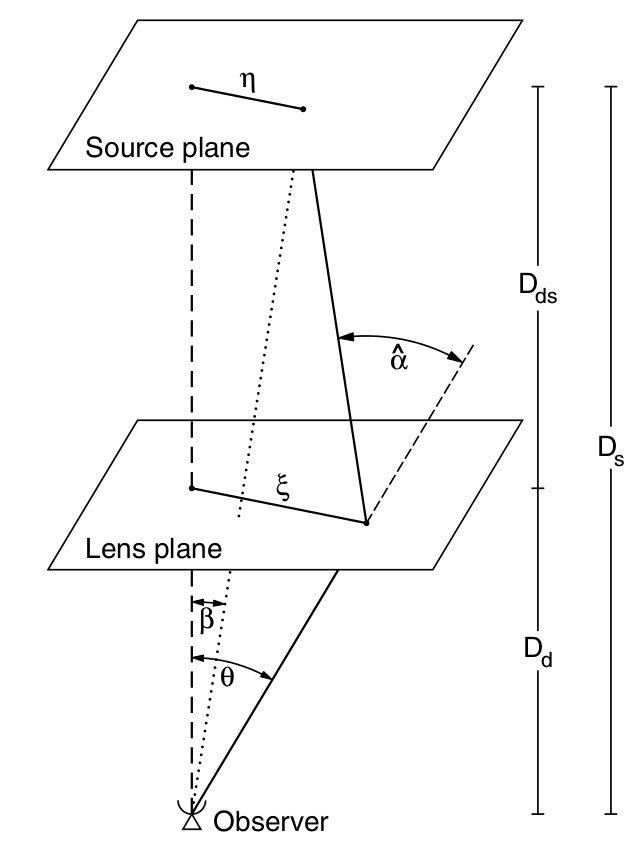
\includegraphics[width=0.5\textwidth]{/home/saas9842/PhD/Lic/figs/Gravitational-lensing-angles}
\caption{The relation between angles and distances in a gravitational lensing setup as described by the lens equation. In this schematic figure, $\eta$ is the position vector of the source with respect to the optical axis of the system, and $\zeta$ is the position vector of the outer surface of the [spherically symmetric] lens (deflector). (Figure from Schneider)}
\end{figure}

Given a certain mass distribution and a fixed $\boldsymbol \xi$, the lens equation can have more than one solution for $\boldsymbol \theta$; each of which corresponds to an image of the source in the sky.  Although obtaining the source position $\eta$ from a given image position $\xi$ using the lens equation is straightforward, finding a general analytical solution for the position of the image(s) of a source at a given position is not. The mapping of $\xi$ to $\eta$ is non--linear. There are, however, analytical models to solve this equation for simple matter distributions on the lens plane such as point--mass, axially symmetric, and elliptical lenses.

The deflection angle due to the surface mass density of the lens gives rise to a deflection potential $\psi$ of the form $\boldsymbol \alpha = \nabla \psi$. Accordingly, another way of presenting the lens equation is in the form of 

\begin{eqnarray}
\label{eq:potential_dimensionless_lensing}
\textbf{y} = \nabla \left(\frac{1}{2}\textbf{x}^2 - \psi(\textbf{x}) \right)
\end{eqnarray}

where $\textbf{x} \equiv \frac{\boldsymbol \xi}{\xi_0}$ and $\textbf{y} \equiv \frac{\boldsymbol \eta}{\eta_0}$ are dimensionless vectors, when $\xi_0$ and $\eta_0$ are length scales in the lens plane and the source plane, respectively. This form of expressing the lens equation leads to the formulation of Fermat's principle in gravitational lensing theory

\begin{eqnarray}
\nabla \phi(\textbf{x}, \textbf{y}) = 0
\end{eqnarray}

where $\phi$ is a scalar function as below

\begin{eqnarray}
\phi(\textbf{x}, \textbf{y}) = \frac{1}{2} (\textbf{x} - \textbf{y})^2 - \psi(\textbf{x})
\end{eqnarray}

Fermat's principle states that the light ray always chooses the path which takes the least \emph{time} to pass through. Therefore, it can be used to relate the time delay between two separate images of a single source to the considered cosmology and mass distribution of the lens.

Light deflection is a propagation phenomenon, influencing only the shape of the light bundle from the source, and not the surface brightness. Therefore, for a monochromatic source, we have the received flux from the source as 

\begin{eqnarray}
\label{eq:flux_to_SB}
S = I_{\nu} d\omega
\end{eqnarray}

where $d\omega$ is the differential solid angle, and $I_{\nu}$ is the monochromatic surface brightness. Since $I_{\nu}$ is not affected by gravitational deflection, the flux changes are merely mirrored in solid angle variation of the image. Hence, the \emph{magnification} due to gravitational lensing is defined as the solid angle ratio of the observed image to that of the non--lensed source

\begin{eqnarray}
\label{eq:mu_domegas}
|\mu| \equiv \frac{d\omega}{d\omega_0}
\end{eqnarray}

On the other hand, the solid angle is related to the angular position of the image (source), via the dimensionless quantities \textbf{x} (\textbf{y}). Therefore, the magnification due to a circularly symmetric lens is given by 

\begin{eqnarray}
\label{eq:mu_beta_theta}
|\mu| = \frac{\theta d\theta}{\beta d\beta}.
\end{eqnarray}

In case of extended sources, we need to solve the lens equation for all points within the source and derive the observed surface brightness distribution in the lens plane $I({\boldsymbol \theta})$ from the true surface brightness distribution in the source plane $I^s({\boldsymbol \beta(\boldsymbol \theta)})$. The lens mapping can be locally linearized and the image distortion written as a Jacobian matrix of 

\begin{eqnarray}
\label{eq:Jacobian}
\mathcal{A}(\boldsymbol \theta) = \frac{\partial \boldsymbol \beta}{\partial \boldsymbol \theta}
\end{eqnarray}

The magnification tensor, -- locally -- mapping the source plane to the image plane for an extended source is then

\begin{eqnarray}
\label{eq:magnification_tensor}
M(\boldsymbol \theta) = \mathcal{A}^{-1}
\end{eqnarray}

whose determinent corresponds to the magnification factor introduced in equation \ref{eq:mu_domegas}, and could be derived from the relative [integrated] fluxes of the images and the source.

\begin{eqnarray}
\label{eq:mu_extended}
\mu = det(M) = \frac{1}{det(\mathcal{A})}
\end{eqnarray}

One of the most interesting and extreme cases of gravitational lensing is the Einstein ring. The lensing setup which gives rise to a complete Einstein ring consists of a point--like source, with a spherically symmetric lens, both of which are collinear with the observer, i.e. the lens is centered at the line of sight between the observer and the source. Therefore, the observer sees a ring--shaped image with an angular radius of $\theta_E$ which is called the angular Einstein radius. This radius, $\theta_E$ is obtained by substituting $\beta=0$ in equation \ref{eq:lens_equation} as:

\begin{eqnarray}
\theta_E = \sqrt{\frac{4GM}{c^2}\frac{D_{ds}}{D_dD_s}}.
\label{eq:lens}
\end{eqnarray}

%<<<<<<< HEAD
 Where $M$ represents the lens mass and $D_d$, $D_s$, and $D_\mathrm{ds}$ are the angular--diameter distances as in Figure \ref{fig:config}. Moreover, as it is immediately concluded from equation \ref{eq:mu_beta_theta}, magnification $\mu$ diverges for the \emph{critical points} where $\beta=0$. The ``infinite'' theoretical magnification points can be mapped into the source plane which gives a set of \emph{caustic curves}. This corresponds to the points where det$(\mathcal{A}) = 0$, and therefore equation \ref{eq:mu_extended} faces division by zero. In reality, however, the finite size of the source keeps the magnification from diverging. The number and relative positions of images of a single source change according to the position of the source with respect to such caustics in the source plane. %%(see figure \hyperref[fig:cusps]{2.2}).
%=======
% Where $M$ represents the lens mass and $D_L$, $D_S$, and $D_\mathrm{LS}$ are the angular--diameter distances as in figure \ref{fig:config}. Moreover, as it is immediately concluded from equation \ref{eq:mu_beta_theta}, magnification $\mu$ diverges for the \emph{critical points} where $\beta=0$. The ``infinite'' theoretical magnification %({\bf explain why infinite magnification is only a theoretical concept}) 
%points can be mapped into the source plane which gives a set of \emph{caustic curves}. The number and relative positions of images of a single source change according to the position of the source with respect to such caustics in the source plane. (see figure \hyperref[fig:cusps]{2.2}).
%>>>>>>> emily

 %% \begin{figure}[ht]
 %% \label{fig:cusps}
 %% \centering
 %% 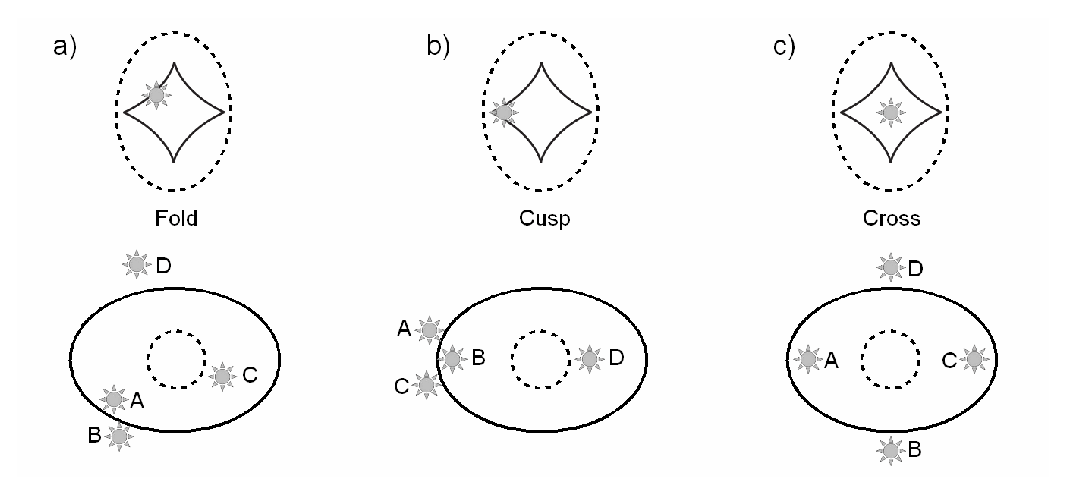
\includegraphics[width=1.0\textwidth]{figs/zack09_4}
 %% \caption{Different configurations of a four-image lens: a) Fold, b) Cusp and c) Cross. The upper row shows the caustics and position of the source (star) in the source plane. The solid line indicates the inner caustic and the dashed line the outer caustic. A source positioned inside the inner caustic produces five images. A source positioned between the inner and outer caustic produces three images, whereas a source positioned outside the outer caustic will not be multiply imaged. In the case of multiple images, one of the images is usually highly de-magnified, so that only four- and two-image lens systems are observed, respectively. The lower row shows the corresponding critical lines and resulting observable images in the lens plane. The inner caustic maps on the outer critical line and vice versa. A close pair (A, B) and a close triplet (A, B, C) are produced in the fold (a) and cusp (b) configurations, respectively. (Figure and caption adopted from \citet{Zackrisson.Riehm2010})}
 %% \end{figure} 

\section{Strong and Weak Lensing}
One observable result of gravitational lensing is magnified (or de-magnified) images of point sources, the other distortions in the images of extended objects. The extent of the lensing effect varies depending on the alignment of the source, the lens and the observer. The closer the center of the lens to the line of sight between the observer and the source, the more significant the image distortion. Therefore, gravitational lensing cases are categorized, according to the level of their magnifications, into two major regimes; \emph{strong} and \emph{weak} lensing. Strong lensing causes dramatic effects such as high magnifications, multiple images, luminous arcs and in some cases even complete Einstein rings. Although strong lensing is a rare effect, it is possible to be detected and studied individually for each case. Weak lensing, on the other hand, occurs when the center of the lens is further away from the observer's line of sight, i.e. $\theta > \theta_E$. Thus the images are weakly magnified or have small distortions. In contrast to strong lensing, weak lensing happens to be very common. Every line of sight is affected by weak lensing at some level hence this effect is detectable through statistical investigations of numerous objects. 

\subsection{Strong Lensing}
As pointed out in the previous section, the lens equation (equation \ref{eq:lens_equation}) can have multiple solutions. Moreover, when the ``thin lens approximation'' is valid, the surface mass density of the lens, i.e. the projected mass of the lens on the lens plane, determines the severity of the gravitational lensing case. Accordingly, one can introduce the constant \emph{critical surface mass density} $\Sigma_{\mathrm{crit}}$ such that for every $\theta$ in the lens equation \ref{eq:lens_equation}, we have $\beta = 0$.

\begin{eqnarray}
\label{eq:Sigma_crit}
\Sigma_c &=& \frac{c^2}{4 \pi G}\frac{D_{os}}{D_{ol} D_{ls}}.
\end{eqnarray}

In cases where $\Sigma > \Sigma_{\mathrm{crit}}$, multiple images from the background source are produced. Exceeding the critical surface mass density may happen only for a part of a specific foreground galaxy or galaxy cluster, the solid angle of which is then called the \emph{strong lensing cross section}. 

On the other hand, the magnification of the image due to the presence of the lens which was defined by equation \ref{eq:mu_domegas}, can also be expressed with the following relation 

\begin{eqnarray}
\label{eq:mu_kappa_gamma}
\mu = \frac{1}{(1 - \kappa)^2 - |\vec{\gamma}|^2}
\end{eqnarray}

which is obtained by substituting the determinant of the Jacobian matrix for the lens equation. In this form, there are two quantities upon which the magnification is dependent, \emph{convergence} $\kappa$ and \emph{shear} vector $\vec{\gamma}$. Convergence, which describes the local isotropic magnification of the source, is a scalar quantity and is defined as the surface mass density of the lens in the unit of the critical surface density as below

\begin{eqnarray}
\label{eq:convergence}
\kappa &\equiv& \frac{\Sigma}{\Sigma_{\mathrm{crit}}}
\end{eqnarray}

 Shear is the measurement of the distortion of the source image and is quantified along each position component on the lens plane, thus a vector. The magnification for point sources is a tensor, only dependent on $\kappa$ and $\vec{\gamma}$, however, for an extended source it is more complicated, depending on the internal surface brightness distribution of the source.

%% \begin{SCfigure}
%%   \centering
%%   \label{fig:shear_convergence}
%%   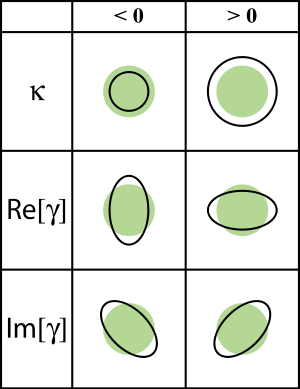
\includegraphics[width=0.3\columnwidth]{figs/shear_convergence}
%%   \caption{from Wikipedia} %https://en.wikipedia.org/wiki/Gravitational_lensing_formalism
%% \end{SCfigure}

\subsection{Strong Lensing Regime}
Strong lensing cases are studied within sub--regimes differing by the angular separation of multiple images produced by each. The angular separation of gravitational lens systems producing multiple images is typically of the order of the Einstein radius of the lens $\theta_E$. Accordingly, the terminology used for various strong lensing separations is

\begin{itemize} 
\item \emph{Macrolensing} refers to cases with typical angular separations, Einstein radii, of the order of \emph{arcseconds}. Macrolensing can be thought of as the combined effect of the dark and luminous matter of an isolated galaxy as well as the effect of galaxy clusters or multiple galaxies along the line of sight. 
\item \emph{Millilensing} (sometimes called \emph{mesolensing}) effects may be produced by satellite galaxies or their dark counterparts, dark matter subhalos, as well as small--scale objects such as intermediate--mass black holes (IMBHs) with typical multiple image separations in the order of \emph{milliarcseconds}. Therefore, lensing effects in this regime potentially address one of the small--scale issues of the CDM theory, the so--called "missing satellites problem", which is mainly the subject of chapter \ref{chap:missing_satellite_problem}. However, the compound effects due to this phenomenon could be in a much larger regime depending on the mass function and spatial distribution of these substructures \citet{Treu10}.
\item \emph{Microlensing} refers to Einstein radii of solar-- and planetary--mass lenses, i.e. the order of \emph{microarcseconds}. Unlike macrolensing and millilensing, microlensing is a transient effect such that it is observable through monitoring a source for a period of time and recording its light curve. The apparent brightness of the source varies over time as the alignment of the lens system changes due to the moving lens. This type of gravitational lensing is not considered in the present study.
\end{itemize}

Following the same convention, strong gravitational lensing cases with smaller angular separations are referred to as nanolensing ($\theta_E \sim 10^{-9}$ arcseconds), picolensing ($\theta_E \sim 10^{-12}$ arcseconds), femtolensing ($\theta_E \sim 10^{-15}$ arcseconds), etc. The terms discussed in the bullet points above are what I mainly use in this thesis.

\subsection{Astrometric Perturbation}
The proximity of the projected image of a foreground massive object to a background source has effects on various angular scales. One effect is a change in the apparent position of the source. This is called the \emph{astrometric effect} and is usually accompanied by magnification or distortion effect. Astrometric effects are, therefore, detectable mostly in dynamic cases, such as microlensing cases where the observer can actually follow the temporal differences in the relative positions in the system. One of these cases stems from the presence of substructures in the main lens such that the deflector consists of a parent halo with a distribution of subhalos inside. 
 
When it comes to the astrometric perturbation due to the substructure inside a halo, the macroimage gets shifted, under the influence of the subhalo, from its original position. This effect is mostly sensitive to intermediate and high mass substructures \citet{Moustakas+2009} and is clearly visible in the results of our modelling in the present work. %%(see Figure \hyperref[fig:astrometric_perturbation]{2.3}). %figure reference is wrong?

%%  \begin{figure}
%% \label{fig:astrometric_perturbation}
%% \centering
%% 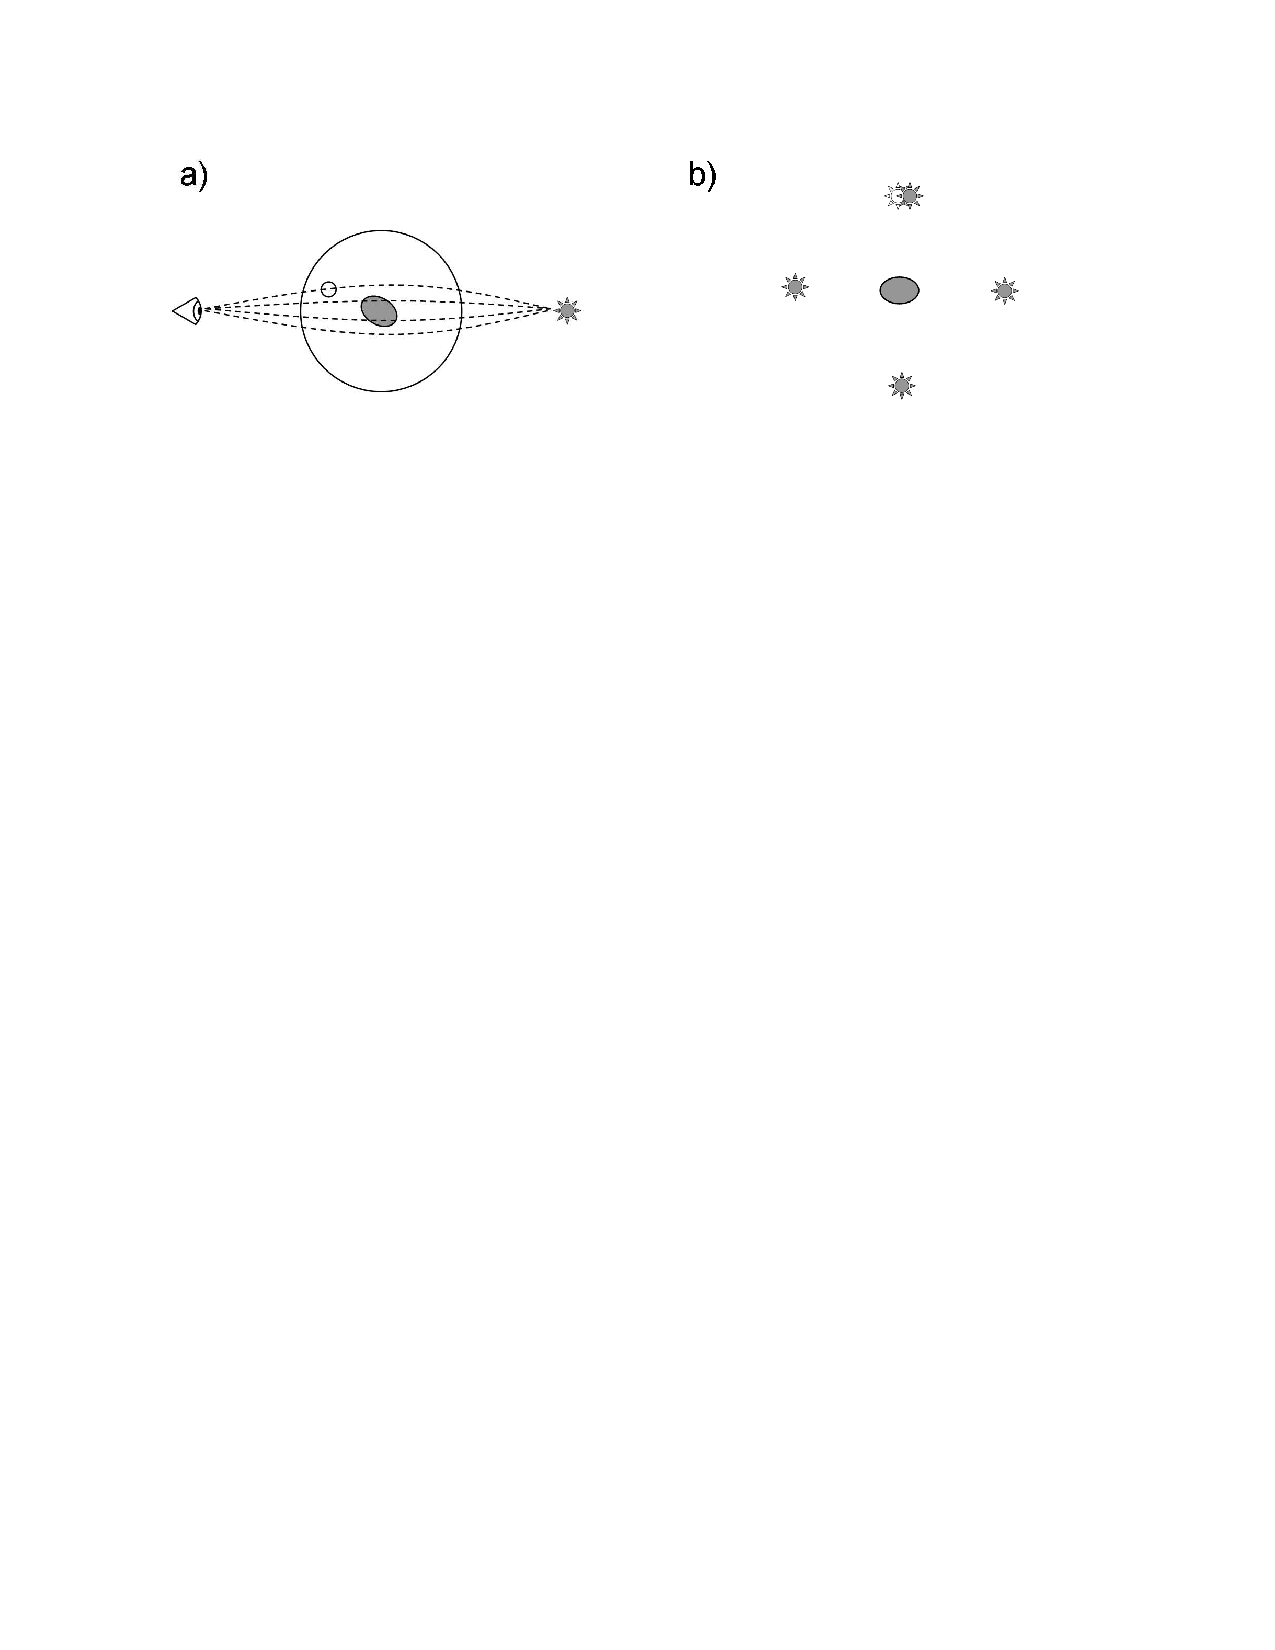
\includegraphics[width=1.0\textwidth]{figs/astrometric_perturbation}
%% \caption {Astrometric perturbations. a) One of the multiple sightlines towards a distant light source passes through a dark subhalo. b) The images of the macro--lensed source are observed at the positions of the gray source symbols. Modeling of the lens system with a smooth lens potential predicts the position of the upper image at the white source symbol. The subhalo close to the sightline of the image causes a deflection on the order of a few tens of milliarcseconds. (Figure and caption adopted from \citet{Zackrisson.Riehm2010}).}
%%  \end{figure}
 
\subsection{Time Delay}
Each macroimage follows a different path to reach the observer, i.e. is subject to a different time delay. This time delay consists of two independent components; the geometrical and the gravitational component. The geometrical term comes from the difference in the light path length for each image. The gravitational component, also known as the \emph{Shapiro} effect, is a relativistic effect of retardation in strong gravitational fields. However, different time delays of various images cannot be observed if the source is not intrinsically variable, since this effect is manifested in the phase difference of the light curves of various images. When it comes to subhalo hunting, the perturbation to the time delays between macroimages predicted by a smooth lens model serves as an evidence for the presence of substructures within the main lens\ignore{ (see Figure \hyperref[fig:time_delay]{2.4})}. As \citet{Moustakas+2009} argue, such an effect is only sensitive to subhalos at the high--mass end of the mass function. Time delay is the only dimensional quantity among the observables of a gravitational lens system, i.e. changes with the length scale of the lens setup. Given two lensing setups which differ in angular--diameter distances, the only variable which breaks the degeneracy of the observables is the time delay of various images.
 
 %% \begin{figure}[h]
 %% \label{fig:time_delay}
 %% \centering
 %% 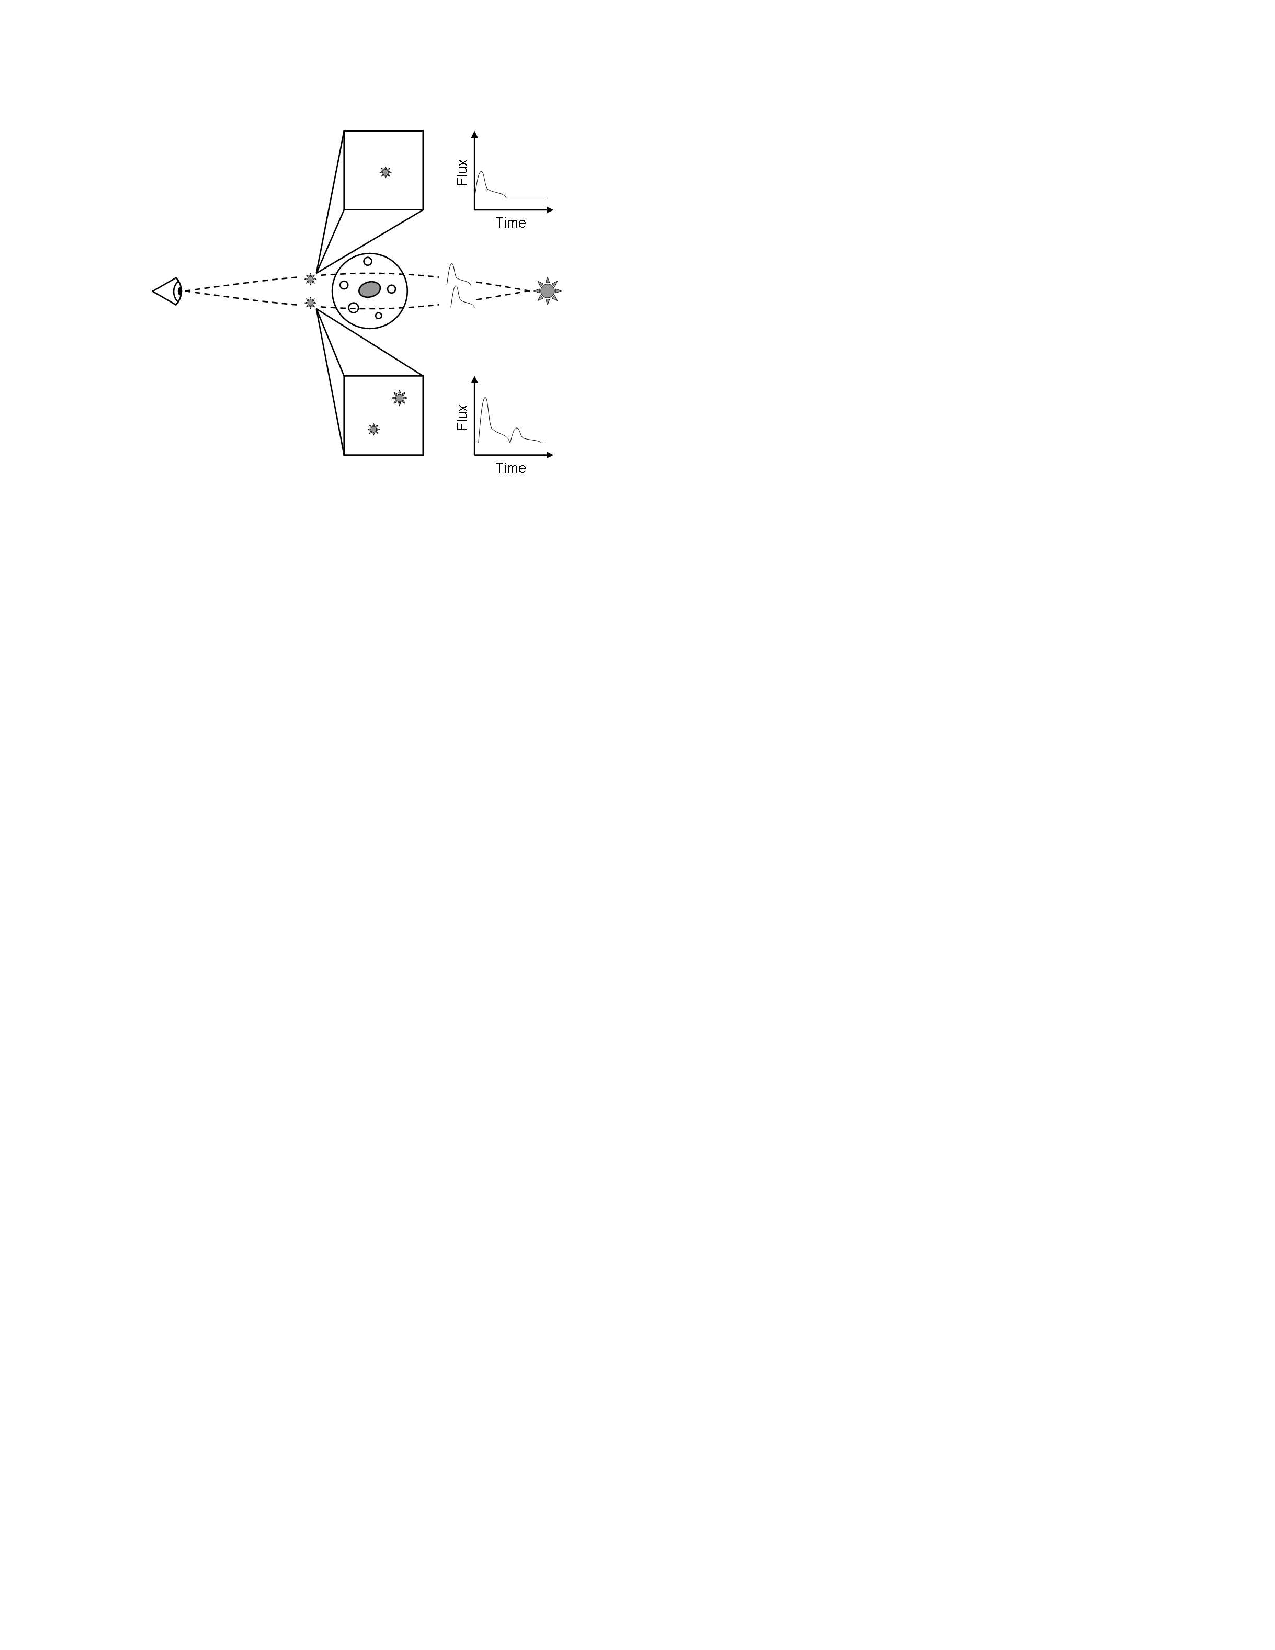
\includegraphics[width=0.5\textwidth]{figs/time_delay}
 %% \caption{A galaxy with a dark matter halo produces distinct macroimages of a background light source. If this source displays intrinsic variability then observable time delays between the different macroimages may occur. If one of the macroimages experiences further small--scale image splitting due to a sub--halo along the line of sight, a light echo may be observable in the affected macroimage. This may serve as a signature of millilensing in cases where the small--scale images blend into one due to insufficient angular resolution. (Figure and caption adopted from \cite{Zackrisson.Riehm2010}.)}
 %% \end{figure}
 
 
\subsection{Flux Ratio Anomalies}
\label{subsec:Flux Ratio Anomalies}
Gravitational lensing is a propagation phenomenon, thus it -- in principle -- conserves the number of photons. On the other hand, the gravitational deflection influences the cross section of the light bundle differentially. Consequently, in order to conserve the flux, the area of the image(s) of the source changes. This leads to different magnifications for different macroimages, as explained in equation \ref{eq:mu_domegas}. However, mere determination of the flux of a single image does not provide any information if the intrinsic flux of the source is unknown. The observable quantities, are rather the flux ratio and positions of two separate macroimages of a single source.

%%  ------------------------  %%
\chapter{Radio interferometry}
In this chapter, I briefly explain the main principles based upon which radio interferometers work. I also try to put radio interferometry into the context of radio astronomy as well as observational astronomy, in general.

\section{Radio telescopes}
A radio telescope is usually made of two main parts:
\begin{itemize}
\item Reflector: The special shape of this reflector, i.e. a parabola, is advantageous compared to concave mirrors -- mostly -- used in reflecting optical telescopes as the parabolic shape keeps all reflected radiation in phase and as I will repeatedly mention in this chapter, coherence is of great importance in radio astronomy. Keeping the same principle in mind, current radio instruments use aperture arrays keeping the electromagnetic wave coherent at the receiver by exerting appropriate delays to the signal. Parabolic antennas are sensitive to a very small area of the sky, i.e. they have high ``directivity'', so an individual antenna is capable of seeing everything in a single pixel.
\item Receiver: Of the main types of receivers used in radio astronomy, i.e. \emph{heterodyne} and \emph{bolometic} receivers, the ones relevant for interferometry are heterodyne receivers. Heterodyne receivers are the most common type of receivers at sub--mm wavelengths (and higher) and they are crucial to use if the signal modulation (both amplitude and phase of the signal) is needed for observations (the case in radio interferometers).
\end{itemize}

%Unlike optical telescopes which scan different points of the focal plain with numerous receivers (pixels of a CCD), radio telescopes generally work with a single receiver at the focal point of their reflector. In other words, radio telescopes see the entire sky (although are not equally sensitive to the whole sky, especially outside the primary beam)\ignore{{\bf primary beam but look it up in the white book!}} within a single pixel only!

%Emily: this is true for dipole antennas but not for parabolic reflectors.  one of the main advantages (that you should also list above) is that parabolic antennas are sensitive to a very small area of sky - i.e. they have high "directivity".  (see the parabolic antenna wikipedia entry if you want.)  so an individual antenna does see everything in a single pixel but not the whole sky.

%Heterodyne receivers are the most common kind of receivers used in radio antennae today, and although in principle they could be arranged in 2--D arrays on the focal plane of the antenna to perform as a CCD in an optical system, the cross--talk among closely placed receivers makes the calibration of each receiver cumbersome and usually inefficient. A more practical approach would be to use several parabolic reflectors (aperture arrays) simultaneously to observe several pointing on the sky.
% Emily: actually, the Westerbork interferometer has APERTIF which is a new focal plane array of receivers.  so maybe these issues are solved now?

%Heterodyne receivers are the most common type of receivers at sub--mm wavelengths (and higher) and they are crucial to use if the signal modulation (both amplitude and phase of the signal) is needed for observations (the case in radio interferometers).\\
% Emily: bolometers don't measure the phase of the EM radiation and they don't have good spectral resolution so they're only good for continuum.  for interferometry you need to know the phase because all of the sub-primary-beam information (the ability to make a map with a resolution that is less than that of the single-antenna beam size) comes from the phase information.

In order to digitally record the electromagnetic wavefront reaching the receiver, the signal needs to be sampled with a frequency at least twice the frequency of the wave (Nyquist theorem). This is an electronically challenging task, and particularly impossible for frequencies in the order of 100 GHz and higher. Therefore, the arriving signal is first mixed with the signal from a stable local oscillator (LO) with a well--known frequency slightly lower than that of the original signal. The mixed signal then has two frequencies $f_\mathrm{sky} + f_\mathrm{LO}$ and $f_\mathrm{sky} - f_\mathrm{LO}$. Therefore, we can sample the low frequency signal with as fine resolution as desired, ignoring the higher frequency. The signal is then demixed by exerting a phase difference and is recorded in two frequency windows below and above the LO frequency, namely the \emph{lower sideband} and the \emph{upper sideband}, by the receiver.

\section{Observational limitations}
Observational limitations of the recorded data may come from the source or, more commonly, from our instruments and can be classified into limitation in 
\begin{itemize}
\item resolution
\item sensitivity
\item dynamic range
\end{itemize}
As will be discussed further into the section, radio interferometry has brought significant improvements in the former two, although mostly at the cost of the latter.

\subsection*{The convolution theorem}
What a radio telescope records is not the direct image of the source at different points at the same time. Rather, a single radio telescope records signals from the primary beam the into a single ``pixel''.  Radio interferometry is based on \emph{the convolution theorem}. According to this theorem, it can be shown that convolving two functions in Fourier space (i.e. Fourier transform of their convolution) is equivalent to multiplying the Fourier transform of the two in the ordinary space.
\begin{align} 
\begin{split}
\mathcal{F}(f*g) &= \mathcal{F}(f) \times \mathcal{F}(g)
\end{split}                    
\end{align}
Where convolution of one function $f(t)$ with another function $g(t)$ means shifting the function $g$ consecutively from $t=-\infty$ to $t=+\infty$, while at each step the multiplication of the two functions (i.e. $f(t)g(t+\tau)$) is added to the convolved function $f*g$:
\begin{align} 
\begin{split}
\mathcal (f*g)(\tau) &= \int_{-\infty}^{+\infty} f(t)g(t+\tau) dt
\end{split}                    
\end{align}
No device can achieve infinite resolution due to its diffraction limit which results in spreading the light from a point source a.k.a. the point spread function (PSF) of the instrument. Anything observed with that instrument will be seen as the convolution of the true source structure with the PSF. Angular resolution of an instrument (i.e. FWHM of its PSF) scales with the size of the aperture and wavelength as $\Delta\theta \propto \lambda / D$. Therefore, the PSF itself scales with the square of the Fourier transform of the aperture which, according to the convolution theorem, equals the Fourier transform of the autocorrelation of the aperture. Therefore, in order to increase the resolving power of an instrument, one needs to either increase the aperture size or decrease the observing wavelength.  Interferometry effectively allows for an increase in the aperature size. While the latter solution might not be possible to arbitrary large extent due to different physical emission mechanisms, the former is one of the reasond for using the interferometry technique.
 
\section{Two-element interferometer}
When we talk about interferometry, clarification is needed to distinguish between the common picture of Young's optical double--slit interferometer and the concepts and techniques used in radio interferometers. In the optical case, the fringe pattern made on the detector plane is a distribution of points with various intensities $I(x) = |E_1(x) + E_2(x)|^2$, and visibility is a real quantity between 0 and 1 defined as below:
\begin{align} 
\begin{split}
V &= \frac{I_\mathrm{max} - I_\mathrm{min}}{I_\mathrm{max} + I_\mathrm{min}}
\end{split}                    
\end{align}
Visibility in the case of radio interferometry, however, is a complex quantity describing the time correlation of the two signals reaching the two elements of the interferometer and can be expressed as below:
\begin{align} 
\begin{split}
\label{eq:vis_def}
V(\tau) &= <E_1(t)E_2^*(t+\tau)>
\end{split}                    
\end{align}
with $\tau$ being the geometrical time delay between the two signals due to the different paths the wave needs to reach each antenna.
\begin{align} 
\begin{split}
\tau &= \frac{\vec{B}.\vec{S}}{c}
\end{split}                    
\end{align}
Where $\vec{B}$ is the three-dimensional distance vector between the two elements, a.k.a. \emph{baseline}, $\vec{S}$ is the source vector and $c$ is the speed of light.

Practically, the time delay $\tau$ of one signal with respect to the other is added to the signal electronically to correct for this effect before sending the two signals to the correlator. Applying the geometrical time delay $\tau$ is equivalent to projecting the baseline connecting the two telescopes on the plane perpendicular to the direction of the source. Therefore, what matters in all math hereafter is the \emph{projected} baseline between the two antennas, rather than the actual baseline. 

The correlated signal is a complex visibility describing the response of the interferometer to the two signals, both amplitude and phase, received from a point source which is a fringe pattern (on the sky) perpendicular to the projected baseline ($BL_\mathrm{proj}$) as seen from that point on the sky. What happens in radio interferometry is that we sample the visibility values on this plane depending on the position of the source, $BL_\mathrm{proj}$, and duration of observations. The interferometer's response to an extended source is simply the superposition of the response patterns of various point sources making up the extended source. In other words, the measured visibility is the integral of source structure multiplied by the response. Therefore,
\begin{align} 
\begin{split}
V_\mathrm{observed} &= \int V^\text{point source}_\text{response} I(x, y) dx dy.
\end{split}                    
\end{align}
Where $x$ and $y$ are celestial coordinates and $I(x, y)$ is the intensity distribution of the extended source.

\subsection*{The van Cittert-Zernike theorem and the interferometer equation}
As long as the source we are observing is far enough that the wavefronts from the source can be approximated as plane waves (i.e. Fraunhofer approximation applies), the complex visibility of the source only depends on the relative position of the two antennae, and the wavelength of the observations. The visibility function, then, is a measure of the spatial coherence of the wavefront of the source encoding the source structure in it.
\begin{align} 
\begin{split}
\label{eq:vC-Z}
V^\mathrm{AB} = <E_A \times E_B^*> = \mathcal{F}(\frac{\vec{R_A} - \vec{R_B}}{\lambda})
\end{split}                    
\end{align}
The left hand side is, by definition, the complex visibility of the source, $\vec{R_A} - \vec{R_B}$ is the observing baseline, and $\mathcal{F}$ is the Fourier transform of the source structure $I(x, y)$. Therefore, rewriting the interferometer equation, one finds:
\begin{align} 
\begin{split}
\label{eq:InterferometerEq}
V(x,y,z) = \int_{x,y} I(x, y) e^{-\frac{-2\pi j}{\lambda}(ux+vy+wz)} \frac{dx dy}{z}
\end{split}                    
\end{align}
where $z=\sqrt{1-x^2-y^2}$. The $wz$ term is made zero by adding a time--delay shift to the signal and if x and y are small enough, the relation above is reduced to a Fourier transform between I(x, y) and V(u, v). This interferometry equation transforms the intensities on the source plane to visibilities on the (u, v) plane and their values depend on the coordinates of the observing baseline, projected on the source plane, as well as the structure of the source and the observing frequency. 

\section{Aperture synthesis}
Back to the definition of visibility in radio interferometry, one can directly conclude that a multi--element interferometer is only a combination of several two--element interferometers, sampling the (u, v) space in pairs, based on their projected baseline and the observing frequency, measuring the visibility at those sample points only. 

\subsection*{Snapshot observations}
Fourier transform is blind to the absolute baseline position, but as baseline is a vector, it does carry information about the direction of the baseline. This implies that in a multi--element interferometer, a [arbitrary] frame of reference is needed for combining the antenna pairs and calculating the transformation from the ordinary plane to the (u, v) plane. The (u, v) coverage in a snapshot is equal to the autocorrelation of the array configuration as seen by the source -- except for the central point which corresponds to the measurement with the hypothetical $BL = 0$, impossible to implement in practice.

Since Fourier transform is a \emph{Hermitian} transformation, a single baseline corresponds to sampling not one, but two points on the visibility plane; one at (u, v), and the other at (-u, -v). Moreover, if I(x, y) is a real number, $V(u, v) = V^*(-u, -v)$. This means that each baseline gives two separate visibility measurements. This means that adding even one more antenna to the array has a significant effect on better sampling the (u, v) plane; one via increasing the number of baselines ($N_\mathrm{BL} = \frac{N_\mathrm{ant}(N_\mathrm{ant}-1)}{2}$), and the other, via double--sampling each baseline as mentioned above. Therefore, a monofrequency snapshot made by an interferometer with $N_\mathrm{ant}$ antennae makes $2N_\mathrm{BL}$ discrete visibility measurements where longer baselines in the (u, v) plane correspond to smaller scales on the image plane and vice--versa. Besides, as seen in equation \ref{eq:InterferometerEq}, the conversion between the (x, y) plane and (u, v) plane is scaled by the observing frequency. Therefore, a wider observing bandwidth results in a wider radial coverage of the (u, v) plane. As (u, v) coordinates are measured in wavelength one way of filling the Fourier space is to observe at multiple wavelengths simultaneously -- given that the sourse looks the same in all these wavelengths. increase the discrete sampling of (u, v) space, closer to a continuous sampling (in the tangential direction), is longer exposure time. In this mode, the Earth rotation leads to a continuous change in projected baselines of the array as seen by the source and hence more (u, v) coverage.

Two extreme regions of the (u, v) plane are usually the most challenging to fill. Long baselines (corresponding to small scales on the image plane) are difficult to achieve for obvious practical reasons and therefore the longest baseline in the array sets the angular resolution of the reconstructed image and obviously the impossibility of infinite baselines make infinite resolution also impossible! On the other hand, short spacings on the (u, v) plane can also be challenging to achieve because of the minimum spacing forced by antenna sizes. This leads to a fundamental feature of any (u, v) sampling known as ``zero-spacing hole''. The lack of visibility measurements on this scale corresponds to missing any smooth large-scale structure of the source. In cases where an unrecovered diffuse component does exist in the original source, the integrated flux of the source measured using the interferometer would be smaller than the integrated flux of the target measured by a single-dish telescope. This is a tell--tale signature of the presence of a large unrecovered structure in the source and is known as ``the missing flux'' problem. The problem arises due to the poor (or lack of) sampling the short spacings on the (u, v) plane. Therefore, the intensity profile of an internally Gaussian source lacks data points in the center thus visibility interpolation tends to flatten out the peak. In many cases, sampling the short spacings with a more compact array or a single--dish telescope helps constrain the light profile of the source.

\subsection*{Aperture synthesis and image reconstruction}
Aperture synthesis is the technique of reconstructing an image from incomplete sampling of the Fourier space. The technique is based on modeling the visibility plane based on the existing samplings. Therefore, the more complete the (u, v) coverage the closer the model image to the real one seen by the array. However, there will always be holes in the sampled (u, v) plane limiting the fidelity and quality (i.e. $\text{dynamic range} = \frac{\text{peak}}{\text{RMS}}$ of the reconstructed image.)

Fourier transform of the (u, v) coverage gives the so-called ``dirty beam'' (equivalent to the point spread function PSF) while the Fourier transform of the measured visibilities on the (u, v) plane results in the ``dirty image'' of the source, which is, as expected, the actual source structure convolved with the dirty beam. Now that we have images of both the beam and the source, we can deconvolve the beam from the image. Remember that deconvolution is non-linear and non-unique! (See \S \ref{sec:CLEAN} on the CLEAN algorithm.)

Modeling is applied while working in the image plane. The process is such that the dirty beam and dirty image are calculated based on the (u, v) coverage and direct visibility measurements, respectively. For this purpose, the (u, v) plane is required to be gridded.\footnote{In fact, this is the issue one faces when using \emph{Fast} Fourier transform (FFT), while \emph{direct} Fourier transform does not require griding the (u, v) plane. One would expect the resulting image to be nearly the same as the model obtained by natural weighting. However, direct FT is so much slower that it is not worth practicing as long as the visibilities are sampled wisely!}. At this step, Nyquist sampling of the (u, v) plane introduces a limitation in the image space, i.e. grid size/cell size needs to  be chosen such that the final PSF includes at least 3 pixels in the image plane. The next step in image reconstruction is deconvolving the beam from the dirty image. The actual interpolation happens here! Deconvolution is not a unique process and hence requires not only griding the (u, v) plane but also making assumptions about the deconvolving beam. One assumption that needs to be made is how to weight the measured visibilities. This question, in turn, has two parts: How are the measured visibilities in one (u, v) pixel weighted? and what is the relative weight of various pixels on the (u, v) plane? Different choices at this step result in different angular resolution and dynamic range limitations in the model image.

\paragraph*{Natural weighting} as it sounds is simply weighting visibilities inversely proportional to the variance of their distribution.
Therefore, short--spacings in the (u, v) plane, with closer samplings, are weighted more than longer baselines which results in higher dynamic range in the modeled image at the cost of angular resolution. In other words, the dirty beam has larger FWHM but less prominent side lobes (compared to the tms noise). Therefore, it is best for imaging faint and smooth sources. 
%natural weighting actually increases sidelobe levels, but what it does is reduce the image rms noise.

\paragraph*{Uniform weighting} is the same as natural weighting with an additional factor inversely proportional to the number of visibilities in each pixel. Therefore, it boosts the contribution from long--spacings by giving the same weight to visibilities at all (u, v) distances, even though those at long distances are sampled more coarsely. This property makes this approach more suitable for sources with rich and complicated structure. Although, the source needs to be bright enough for this approach to work best. This is because this weighting scheme results in a narrow(er than naturally--weighted) PSF with smaller side lobes and therefore, better angular resolution. However, the RMS of the residuals of this model tends are large(r than that of natural by at least an order of $\sim 2$), i.e. poorer sensitivity.

\paragraph*{Briggs weighting} is a tunable combination of both approaches above. The tunability of Briggs' recipe is applied through the \emph{robust} parameter. This parameter changes in the range of -2 to +2 from uniform to natural weighting. Usually, robust=0.5 gives a good compromise between the two extreme approaches. Although it still depends on the preferences based on the scientific target.

\paragraph*{(u, v) tapering} is useful when the observed source is extended and most of the information lies in short baselines. Therefore, in order to improve the sensitivity to emission at larger spatial scales, we can overweight the measurements made using these baselines even further and decrease the weight of measurements where we have a lower signal, i.e. long baselines. This can be done via Gaussian circular tapers in the (u, v) plane. If the source has a very extended structure, which is remained unrecovered due to the short--spacing hole in the (u, v) coverage, even with natural weighting, then (u, v) tapering is the last resort to recover that diffuse emission. 

As a matter of fact, one might want to get rid of an extended emission they are not interested in, and focus more on the small--scale clumpy structure of their source. In which case, one only needs to apply an inverse Gaussian taper to the (u, v) plane.

The method used in {\bf Paper II} is based on combining different weightings of the same measurement set to put emphasis on features with different angular scales. 

\subsection*{CLEAN algorithm and deconvolving the dirty beam}
\label{sec:CLEAN}
While interferometry data are incomplete due to lack of information on some spatial frequencies, we can interpolate the (u, v) plane by applying our prior information about the source structure as the criteria required to proceed with deconvolution. Clearly, the more our prior information about the source, the more reliable the model image is.

The problem of deconvolving the dirty beam from the dirty image has non--unique solutions. An intuitive way to show this is to assume a source with non--zero visibilities everywhere but where we are making our measurements, i.e. our (u, v) coverage. This class of sources remain invisible to the interferometer, as long as the (u, v) coverage is the same. Now, one can add \emph{any} combination of these ``invisible'' sources to our reconstructed image without the measurement set changing. Improving the (u, v) coverage will decrease the number of these combinations and therefore, increase the image fidelity and yet \emph{high} fidelity is not the same as \emph{infinite} fidelity. Therefore, the reconstructed image always remains a model of our real data.

CLEAN \citep[][]{Hogbom1974} is the oldest, fastest and best deconvolution algorithm practiced today for image reconstruction in radio interferometry. This algorithm starts at the maximum flux point in the image, subtracts the PSF at that point and adds a 2-D Gaussian component (with the same FWHM of the PSF and scaled flux) to the CLEAN image instead. The algorithm then repeats these three steps for the peak in the residual map until either of the criteria below is met: 
\begin{itemize}
\item Noise limit: If the peak in the residual map has a smaller value than $\alpha \sigma_\mathrm{RMS}$
\\($\alpha$ is an arbitrary coefficient set by the scientific purpose of the image.)
\item Dynamic range limit: If the peak in the residual map has a smaller value than $\frac{1}{\alpha} \times f_\mathrm{max}$ of the dirty beam
\item Maximum number of CLEAN cycles, which is an experimental (arbitrary) criterion.
\end{itemize}

Finally, what the algorithm produces are three matrices below:
\paragraph*{CLEAN model:} A set of point sources subtracted from the dirty image where flux peaks are located.
\paragraph*{CLEAN beam:} The corresponding Gaussian to the dirty beam. In other words, the PSF model. If the dirty beam is elliptical, then the CLEAN beam is also a similarly--elliptical Gaussian.
\paragraph*{CLEAN image:} It is simply the CLEAN model convolved with the CLEAN beam and is the final product of the image reconstruction procedure. 


While different deconvolution algorithms apply different criteria to the source structure, the CLEAN algorithm's basic assumption is that the source is made of discrete Dirac delta functions, i.e. point sources. Therefore, it tends to convert smooth and diffused components into clumpy ones. While one does not loose real emission by not CLEANing it, it is possible to get artificial features by CLEANing noise!

The current commonly--used implementation of CLEAN is the Cotton--Schwab CLEAN which consists of two same--level, linked cycles.
Start with a {\bf Minor cycle} as below:
\begin{enumerate}
\item Locate the peak intensity in the dirty image.
\item\begin{enumerate}
    \item Subtract a dirty beam centering at the point of the peak, from the dirty image.
    \item Compute the residual image = image used in step (1) -- product of (2.a).
    \item Scale down the flux density in residual image to {\bf g} times the image peak, where {\bf g} is the arbitrary CLEAN gain value.
    \end{enumerate}
\item\begin{enumerate}
    \item Add a point--like component to the CLEAN model, at the position of the peak.
    \item Set the flux density of the point in CLEAN model to the peak of the PSF.
    \item Convolve the newly--added point of the CLEAN model with the CLEAN beam and add it to the CLEAN image
    \end{enumerate}
\item Use the product of step (2.b) in step (1). 
\end{enumerate}
A {\bf Major cycle}, then, follows the minor cycle as below:
\begin{enumerate}
\item Compute model visibilities corresponding to the CLEAN model made in the minor cycle.
\item Compute the residual visibilities = observed visibilities -- model visibilities made in step(1).
\item FFT the residual visibilities and feed it to the next minor cycle 
\end{enumerate}

While the CLEANing process seems complete within the minor cycle, the major cycle is needed because the algorithm (minor cycle only) cannot subtract anything from marginal parts of the image where we have no information about possible sources in those regions whose side lobes (only!) affect our dirty image.

%%  ------------------------  %%
\chapter{Summary}
With the fast improvement of observational facilities the required angular resolution and sensitivity for the discovery of compound lens systems is becoming available. Given all the uncertainties concerning the existence, abundance, mass function, and inner mass distribution of dark matter substructure, it is important to estimate the alignment probabilities of lens substructures combined with the detection limits. It is important to keep in mind that with a detailed picture of model expectations at hand even null detections provide constraints on the background model.

In {\bf Paper I} we use simulations of strongly lensed quasar jets as expected by three different VLBI configurations and receivers to probe dark matter substructure. The dark matter substructure in this Paper Is assumed to consist of intermediate--mass black holes (i.e. point--like) and ultracompact minihalos ($\rho \propto r^{-2.5}$) within the main lens at $z \simeq 0.5$. We demonstrate that small--scale morphological distortions in one of the macroimages -- that is not replicated in others in a large number of macrolensed jet systems with the expected (submilliarcsecond) resolution of the array is used to set constraints on detection limits of such substructures and their abundance. We argue that intermediate--mass black holes with $M_\mathrm{IMBH} \sim 10^3$--$10^6\ $ \msun  are detectable and therefore, non--detections of such distortions rule out their contribution in the surface mass fraction down to $f_\mathrm{IMBH}\gtrsim 0.01$ in the dark matter halo of the main lens at the position of the macroimage. The same investigation for ultracompact minihalos (that have a central density slope slightly steeper than the isothermal profile $\rho\sim r^{-2.5}$) places a constraint of $f_\mathrm{UCMH}\gtrsim 0.1$ on their contribution to the dark matter budget of the main lens. While we show that standard CDM halos (with NFW density profile) with $M_\mathrm{FNW} \simeq 10^8\ $ \msun  also produce detectable distortions due to the far shallower central density profile ($\rho \propto r^{-1}$), their effective lensing cross section is too small for the probability of successful alignments to be of any interest ($P_\mathrm{milli}\sim 10^{-4}$).

The extremely low probability of proper alignment for standard CDM subhalos presented in {\bf Paper I}, brings us to {\bf Paper II} in which we adopt a similar approach to investigate small--scale perturbations using simulations of multiply--lensed sub--mm galaxies (SMGs).  These sources provide 10-100 times more coverage of the lens plane. This Paper Investigates simulations of compound lens systems where the lensed source is a dust starforming galaxy at $z = 2$ where ALMA band 7, 8, and 9 (with frequency coverage between 275 -- 720 GHz) probes the dust continuum emission of the source with submilliarcsecond angular resolution.  We aim for lens perturbers of $M_\mathrm{sub} = 10^5 - 10^{10} $ \msun  in a Milky Way--sized halo.  This is the relevant mass range for both the ``missing satellite problem'' \ref{subsec:missing-satellite} and the ``core--cusp problem'' \ref{subsec:core-cusp}. The analysis in this paper uses different weighting schemes for simulated complex visibilities and instrumental noise effects are taken into account. We use not only the local (small--scale) lens effects of substructures but also the astrometric shift of the main lens solution to place constraints on the presence, mass and central density slope of the lens perturber (substructure). In this paper, we demonstrate that SIS perturbers down to $M_\mathrm{vir} \approx 3\times 10^7 $ \msun  will be detectable with 2hr observations with the full ALMA array. Moreover, we argue that while these observations could, in principle, be used to tell the difference between the observational signature of a compact SIS and a lens subhalo with NFW (or Einasto) profile, the shape parameter ($\alpha_\mathrm{Ein}$ for Einasto or $\gamma$ in general NFW) remains highly degenerate with the subhalo mass. In the end of {\bf Paper II} we draw attention to different mass definitions used in lens modelings ($M_\mathrm{einstein}$, the projected mass within the Einstein radius of the lens) and cosmological simulations ($M_\mathrm{tidal}$, the 3D tidally--truncated mass of a subhalo that is being dissolved (?!) in the parent halo) to argue that the conversion between the two strongly depends on the assumptions made in the process of deprojection. 



% \bibliographystyle{aa}  % style aa.bst
% \bibliography{myattempt.bib}  % your references Yourfile.bib
 
% attach the PDF to the paper here 
%\includepdf[pages={-}]{sandbergetal2012.pdf}  % does not work :(

\begin{thebibliography}{}
\bibitem[\protect\citeauthoryear{Alcock et al.}{1998}]{Alcock+1998} 
Alcock C., et al., 1998, ApJ, 499, L9 
\bibitem[\protect\citeauthoryear{Angulo 
\& White}{2010}]{Angulo.White2010} Angulo R.~E., White S.~D.~M., 2010, MNRAS, 405, 143 
\bibitem[\protect\citeauthoryear{Angulo 
\& White}{2010}]{Angulo.White2010} Angulo R.~E., White S.~D.~M., 2010, MNRAS, 401, 1796 
\bibitem[\protect\citeauthoryear{B{\oe}hm et 
al.}{2014}]{Boem+2014} B{\oe}hm C., Schewtschenko J.~A., 
Wilkinson R.~J., Baugh C.~M., Pascoli S., 2014, MNRAS, 445, L31 
\bibitem[\protect\citeauthoryear{Begeman}{1989}]{Begeman1989} Begeman K.~G., 1989, A\&A, 223, 47 
\bibitem[\protect\citeauthoryear{Bekenstein}{2004}]{Bekenstein2004} 
Bekenstein J.~D., 2004, PhRvD, 70, 083509 
\bibitem[\protect\citeauthoryear{Bellazzini et 
al.}{2013}]{Bellazzini+2013} Bellazzini M., Oosterloo T., Fraternali F., Beccari G., 2013, A\&A, 559, L11 
\bibitem[\protect\citeauthoryear{Bennett et 
al.}{2013}]{WMAP9} Bennett C.~L., et al., 2013, ApJS, 208, 20 
\bibitem[\protect\citeauthoryear{Bergstr{\"o}m}{2013}]{Bergstrom2013} 
Bergstr{\"o}m L., 2013, PhST, 158, 014014
\bibitem[\protect\citeauthoryear{Bloomfield}{2013}]{Bloomfield2013} 
Bloomfield J.~K., 2013, PhDT, 
\bibitem[\protect\citeauthoryear{Bosma}{1981}]{Bosma1981} Bosma 
A., 1981, AJ, 86, 1825 
\bibitem[\protect\citeauthoryear{Boylan-Kolchin, Bullock, 
\& Kaplinghat}{2012}]{Boylan-Kolchin+2012} Boylan-Kolchin M., Bullock J.~S., Kaplinghat M., 2012, MNRAS, 422, 1203 
\bibitem[\protect\citeauthoryear{Boylan-Kolchin, Bullock, 
\& Kaplinghat}{2011}]{Boylan-Kolchin+2011} Boylan-Kolchin M., Bullock J.~S., Kaplinghat M., 2011, MNRAS, 415, L40 
\bibitem[\protect\citeauthoryear{Bringmann}{2009}]{Bringmann2009} 
Bringmann T., 2009, NJPh, 11, 105027 
\bibitem[\protect\citeauthoryear{Brooks et al.}{2013}]{Brooks+2013} 
Brooks A.~M., Kuhlen M., Zolotov A., Hooper D., 2013, ApJ, 765, 22 
\bibitem[\protect\citeauthoryear{Bullock et 
al.}{2001}]{Bullock+2001} Bullock J.~S., Kolatt T.~S., Sigad Y., 
Somerville R.~S., Kravtsov A.~V., Klypin A.~A., Primack J.~R., Dekel A., 
2001, MNRAS, 321, 559 
\bibitem[\protect\citeauthoryear{Bullock, Kravtsov, 
\& Weinberg}{2000}]{Bullock+2000} Bullock J.~S., Kravtsov A.~V., Weinberg D.~H., 2000, ApJ, 539, 517 
\bibitem[\protect\citeauthoryear{Bullock et 
al.}{2010}]{Bullock+2010} Bullock J.~S., Stewart K.~R., Kaplinghat 
M., Tollerud E.~J., Wolf J., 2010, ApJ, 717, 1043 
\bibitem[\protect\citeauthoryear{Cautun et al.}{2015}]{Cautun+2015} 
Cautun M., Wang W., Frenk C.~S., Sawala T., 2015, MNRAS, 449, 2576
\bibitem[\protect\citeauthoryear{Clifton}{2006}]{Clifton2006} 
Clifton T., 2006, PhDT
\bibitem[\protect\citeauthoryear{Clifton et 
al.}{2012}]{Clifton+2012} Clifton T., Ferreira P.~G., Padilla A., 
Skordis C., 2012, PhR, 513, 1  
\bibitem[\protect\citeauthoryear{Clowe et al.}{2006}]{Clowe+2006} 
Clowe D., Brada{\v c} M., Gonzalez A.~H., Markevitch M., Randall S.~W., 
Jones C., Zaritsky D., 2006, ApJ, 648, L109
\bibitem[\protect\citeauthoryear{Del Popolo et 
al.}{2014}]{DelPopolo+2014} Del Popolo A., Lima J.~A.~S., Fabris 
J.~C., Rodrigues D.~C., 2014, JCAP, 4, 021 
\bibitem[\protect\citeauthoryear{Del Popolo}{2014}]{DelPopolo2014} 
Del Popolo A., 2014, IJMPD, 23, 1430005  
\bibitem[\protect\citeauthoryear{Di Cintio et 
al.}{2014}]{DiCintio+2014} Di Cintio A., Brook C.~B., Dutton A.~A., 
Macci{\`o} A.~V., Stinson G.~S., Knebe A., 2014, MNRAS, 441, 2986 
\bibitem[\protect\citeauthoryear{Doroshkevich, Shandarin, 
\& Saar}{1978}]{Doroshkevich+1978} Doroshkevich A.~G., Shandarin S.~F., Saar E., 1978, MNRAS, 184, 643 
\bibitem[\protect\citeauthoryear{Dubinski 
\& Carlberg}{1991}]{Dubinski.Carlberg1991} Dubinski J., Carlberg R.~G., 1991, ApJ, 378, 496 
\bibitem[\protect\citeauthoryear{Dutton 
\& Macci{\`o}}{2014}]{Dutton.Maccio2014} Dutton A.~A., Macci{\`o} A.~V., 2014, MNRAS, 441, 3359 
\bibitem[\protect\citeauthoryear{Eddington}{1919}]{Eddington1919} 
Eddington A.~S., 1919, Natur, 104, 372
\bibitem[\protect\citeauthoryear{Einasto}{1965}]{Einasto1965} 
Einasto J., 1965, TrAlm, 5, 87
\bibitem[\protect\citeauthoryear{Einasto et 
al.}{1974}]{Einasto+1974} Einasto J., Saar E., Kaasik A., Chernin 
A.~D., 1974, Natur, 252, 111 
\bibitem[\protect\citeauthoryear{Einstein}{1911}]{Einstein1911} 
Einstein A., 1911, AnP, 340, 898 
\bibitem[\protect\citeauthoryear{Famaey}{2015}]{Famaey2015} Famaey 
B., 2015, arXiv, arXiv:1501.01788 
\bibitem[\protect\citeauthoryear{Famaey 
\& McGaugh}{2012}]{Famaey.McGaugh2012} Famaey B., McGaugh S.~S., 2012, LRR, 15, 10 
\bibitem[\protect\citeauthoryear{Ferrero et 
al.}{2012}]{Ferrero+2012} Ferrero I., Abadi M.~G., Navarro J.~F., 
Sales L.~V., Gurovich S., 2012, MNRAS, 425, 2817
\bibitem[\protect\citeauthoryear{Gao et al.}{2008}]{Gao+2008} 
Gao L., Navarro J.~F., Cole S., Frenk C.~S., White S.~D.~M., Springel V., 
Jenkins A., Neto A.~F., 2008, MNRAS, 387, 536
\bibitem[\protect\citeauthoryear{Garrison-Kimmel et 
al.}{2014}]{Garrison-Kimmel+2014} Garrison-Kimmel S., Boylan-Kolchin M., 
Bullock J.~S., Kirby E.~N., 2014, MNRAS, 444, 222  
\bibitem[\protect\citeauthoryear{Gelmini}{2015}]{TASI2014} 
Gelmini G.~B., 2015, arXiv, arXiv:1502.01320
\bibitem[\protect\citeauthoryear{Gil-Mar{\'{\i}}n et 
al.}{2015}]{SDSS} Gil-Mar{\'{\i}}n H., et al., 2015, MNRAS, 
452, 1914  
\bibitem[\protect\citeauthoryear{Griest, Cieplak, 
\& Lehner}{2014}]{Griest+2014} Griest K., Cieplak A.~M., Lehner M.~J., 2014, ApJ, 786, 158
\bibitem[\protect\citeauthoryear{Guo et al.}{2011}]{Guo+2011} 
Guo Q., et al., 2011, MNRAS, 413, 101 
\bibitem[\protect\citeauthoryear{H{\"o}gbom}{1974}]{Hogbom1974} H{\"o}gbom J.~A., 1974, A\&AS, 15, 417  
\bibitem[\protect\citeauthoryear{Hannestad}{2004}]{Hannestad2004} 
Hannestad S., 2004, PhRvD, 70, 043506 
\bibitem[\protect\citeauthoryear{Hayashi 
\& White}{2008}]{Hayashi.White2008} Hayashi E., White S.~D.~M., 2008, MNRAS, 388, 2 
\bibitem[\protect\citeauthoryear{Hu, Barkana, 
\& Gruzinov}{2000}]{Hu+2000} Hu W., Barkana R., Gruzinov A., 2000, PhRvL, 85, 1158 
\bibitem[\protect\citeauthoryear{Ibata et al.}{2013}]{Ibata+2013} 
Ibata R.~A., et al., 2013, Natur, 493, 62
\bibitem[\protect\citeauthoryear{Kirby et al.}{2014}]{Kirby+2014} 
Kirby E.~N., Bullock J.~S., Boylan-Kolchin M., Kaplinghat M., Cohen J.~G., 
2014, MNRAS, 439, 1015  
\bibitem[\protect\citeauthoryear{Klypin et al.}{2015}]{Klypin+2015} 
Klypin A., Karachentsev I., Makarov D., Nasonova O., 2015, MNRAS, 454, 1798 
\bibitem[\protect\citeauthoryear{Klypin et al.}{1999}]{Klypin+1999} 
Klypin A., Kravtsov A.~V., Valenzuela O., Prada F., 1999, ApJ, 522, 82 
\bibitem[\protect\citeauthoryear{Kroupa et 
al.}{2010}]{Kroupa+2010} Kroupa P., et al., 2010, A\&A, 523, A32 
\bibitem[\protect\citeauthoryear{Kroupa, Theis, 
\& Boily}{2005}]{Kroupa+2005} Kroupa P., Theis C., Boily C.~M., 2005, A\&A, 431, 517 
\bibitem[\protect\citeauthoryear{Kuhlen, Vogelsberger, 
\& Angulo}{2012}]{Kuhlen+2012} Kuhlen M., Vogelsberger M., Angulo R., 2012, PDU, 1, 50 
\bibitem[\protect\citeauthoryear{M{\"u}ller, Jerjen, 
\& Binggeli}{2015}]{Muller+2015} M{\"u}ller O., Jerjen H., Binggeli B., 2015, A\&A, 583, A79 
\bibitem[\protect\citeauthoryear{Macci{\`o}, Dutton, 
\& van den Bosch}{2008}]{Maccio+2008} Macci{\`o} A.~V., Dutton A.~A., van den Bosch F.~C., 2008, MNRAS, 391, 1940 
\bibitem[\protect\citeauthoryear{McGaugh}{2015}]{McGaugh2015} 
McGaugh S.~S., 2015, CaJPh, 93, 250 
\bibitem[\protect\citeauthoryear{Melott et al.}{1983}]{Melott+1983} 
Melott A.~L., Einasto J., Saar E., Suisalu I., Klypin A.~A., Shandarin 
S.~F., 1983, PhRvL, 51, 935 
\bibitem[\protect\citeauthoryear{Metz, Kroupa, 
\& Jerjen}{2009}]{Metz+2009} Metz M., Kroupa P., Jerjen H., 2009, MNRAS, 394, 2223 
\bibitem[\protect\citeauthoryear{Milgrom}{1983}]{Milgrom1983} 
Milgrom M., 1983, ApJ, 270, 365 
\bibitem[\protect\citeauthoryear{Moore et al.}{1999}]{Moore+1999} 
Moore B., Ghigna S., Governato F., Lake G., Quinn T., Stadel J., Tozzi P., 
1999, ApJ, 524, L19 
\bibitem[\protect\citeauthoryear{Moustakas et 
al.}{2009}]{Moustakas+2009} Moustakas L.~A., et al., 2009, astro, 
2010, 214 
\bibitem[\protect\citeauthoryear{Navarro et 
al.}{2004}]{Navarro+2004} Navarro J.~F., et al., 2004, MNRAS, 349, 
1039
\bibitem[\protect\citeauthoryear{Navarro, Frenk, 
\& White}{1997}]{NFW} Navarro J.~F., Frenk C.~S., White S.~D.~M., 1997, ApJ, 490, 493
\bibitem[\protect\citeauthoryear{Navarro, Frenk, 
\& White}{1996}]{NFW96} Navarro J.~F., Frenk C.~S., White S.~D.~M., 1996, ApJ, 462, 563 
\bibitem[\protect\citeauthoryear{Navarro et 
al.}{2010}]{Navarro+2010} Navarro J.~F., et al., 2010, MNRAS, 402, 
21
\bibitem[\protect\citeauthoryear{Ostriker, Peebles, 
\& Yahil}{1974}]{Ostriker+1974} Ostriker J.~P., Peebles P.~J.~E., Yahil A., 1974, ApJ, 193, L1 
\bibitem[\protect\citeauthoryear{Papastergis et 
al.}{2015}]{Papastergis+2015} Papastergis E., Giovanelli R., Haynes M.~P., Shankar F., 2015, A\&A, 574, A113 
\bibitem[\protect\citeauthoryear{Pawlowski, Kroupa, 
\& Jerjen}{2013}]{Pawlowski+2013} Pawlowski M.~S., Kroupa P., Jerjen H., 2013, MNRAS, 435, 1928 
\bibitem[\protect\citeauthoryear{Pawlowski 
\& McGaugh}{2014}]{Pawlowski.McGaugh2014} Pawlowski M.~S., McGaugh S.~S., 2014, MNRAS, 440, 908 
\bibitem[\protect\citeauthoryear{Pawlowski, McGaugh, 
\& Jerjen}{2015}]{Pawlowski+2015} Pawlowski M.~S., McGaugh S.~S., Jerjen H., 2015, MNRAS, 453, 1047 
\bibitem[\protect\citeauthoryear{Percival et 
al.}{2002}]{2dFGRS} Percival W.~J., et al., 2002, MNRAS, 337, 
1068 
\bibitem[\protect\citeauthoryear{Perlmutter et 
al.}{1999}]{Perlmutter+1999} Perlmutter S., et al., 1999, ApJ, 517, 565 
\bibitem[\protect\citeauthoryear{Phillips et 
al.}{2015}]{Phillips+2015} Phillips J.~I., Cooper M.~C., Bullock 
J.~S., Boylan-Kolchin M., 2015, MNRAS, 453, 3839 
\bibitem[\protect\citeauthoryear{Planck Collaboration et 
al.}{2015}]{Planck2015} Planck Collaboration, et al., 2015, arXiv, 
arXiv:1502.01589 
\bibitem[\protect\citeauthoryear{Riess et al.}{1998}]{Riess+1998} 
Riess A.~G., et al., 1998, AJ, 116, 1009 
\bibitem[\protect\citeauthoryear{Rubin 
\& Ford}{1970}]{Rubin.Ford1970} Rubin V.~C., Ford W.~K., Jr., 1970, IAUS, 38, 61
\bibitem[\protect\citeauthoryear{Rubin, Thonnard, 
\& Ford}{1978}]{Rubin+1978} Rubin V.~C., Thonnard N., Ford W.~K., Jr., 1978, ApJ, 225, L107 
\bibitem[\protect\citeauthoryear{Sawala et al.}{2015}]{Sawala+2015} 
Sawala T., et al., 2015, arXiv, arXiv:1511.01098 
\bibitem[\protect\citeauthoryear{Sawala et al.}{2014}]{Sawala+2014} 
Sawala T., et al., 2014, arXiv, arXiv:1412.2748 
\bibitem[\protect\citeauthoryear{Tollerud, Boylan-Kolchin, 
\& Bullock}{2014}]{Tollerud+2014} Tollerud E.~J., Boylan-Kolchin M., Bullock J.~S., 2014, MNRAS, 440, 3511 
\bibitem[\protect\citeauthoryear{Treu}{2010}]{Treu2010} Treu T., 2010, ARA\&A, 48, 87 
\bibitem[\protect\citeauthoryear{Tully et al.}{2015}]{Tully+2015} 
Tully R.~B., Libeskind N.~I., Karachentsev I.~D., Karachentseva V.~E., 
Rizzi L., Shaya E.~J., 2015, ApJ, 802, L25
\bibitem[\protect\citeauthoryear{Vera-Ciro et 
al.}{2013}]{Vera-Ciro+2013} Vera-Ciro C.~A., Helmi A., Starkenburg E., 
Breddels M.~A., 2013, MNRAS, 428, 1696 
\bibitem[\protect\citeauthoryear{Walker 
\& Pe{\~n}arrubia}{2011}]{Walker.Penarrubia2011} Walker M.~G., Pe{\~n}arrubia J., 2011, ApJ, 742, 20  
\bibitem[\protect\citeauthoryear{Walsh, Carswell, 
\& Weymann}{1979}]{Walsh+1979} Walsh D., Carswell R.~F., Weymann R.~J., 1979, Natur, 279, 381 
\bibitem[\protect\citeauthoryear{Yoo, Chanam{\'e}, 
\& Gould}{2004}]{Yoo+2004} Yoo J., Chanam{\'e} J., Gould A., 2004, ApJ, 601, 311 
\bibitem[\protect\citeauthoryear{Zackrisson 
\& Riehm}{2010}]{Zackrisson.Riehm2010} Zackrisson E., Riehm T., 2010, AdAst, 2010, 478910 
\bibitem[\protect\citeauthoryear{Zwicky}{1937}]{Zwicky1937} Zwicky 
F., 1937, ApJ, 86, 217 
\bibitem[\protect\citeauthoryear{Zwicky}{1933}]{Zwicky1933} Zwicky 
F., 1933, AcHPh, 6, 110
\end{thebibliography}
\end{document}
